%%%%%%%%%%%%%%%%%%%%%%%%%%%%%%%%%%%%%%%%%%%%%%%%%%%%%%%%%%%%%%%%%%%%%%%%%%%
%
% Template für Diplomarbeiten 
% (im speziellen für Diplomarbeiten an der Universität Stuttgart)
%
% Copyright (c) 2005 by Tim Schönleber
%
% This template is free; you can redistribute it and/or modify
% it under the terms of the GNU General Public License as published by
% the Free Software Foundation; either version 2 of the License, or
% (at your option) any later version.
%
% This program is distributed in the hope that it will be useful,
% but WITHOUT ANY WARRANTY; without even the implied warranty of
% MERCHANTABILITY or FITNESS FOR A PARTICULAR PURPOSE. See the
% GNU General Public License for more details.
%
% You should have received a copy of the GNU General Public License
% along with this program; if not, write to the Free Software
% Foundation, Inc., 59 Temple Place, Suite 330, Boston, MA 02111-1307 USA
%
% Author: Tim Schönleber
% Datum: 11.04.2005
% Version: 1.0
%
%%%%%%%%%%%%%%%%%%%%%%%%%%%%%%%%%%%%%%%%%%%%%%%%%%%%%%%%%%%%%%%%%%%%%%%%%%%

\documentclass[paper=a4,       % Papiergröße A4
					 11pt,
					 BCOR0mm,  % Bindekorrektur
					 DIV10,    % Satzspiegel mit 10er-Teilung
					 automark, % lebende Kolumnentitel
					 twoside,
					 halfparskip,
					 bibtotoc,
					 headsepline,
					 normalheadings,
					 appendixprefix,
					 pagesize  % Seitengröße wird bei dvi und pdf richtig gesetzt
 ]{scrbook}

% gängige Standardpakete
\usepackage[english]{babel}
\usepackage{graphicx}
\usepackage{microtype}
\usepackage{url}
\usepackage{mparhack, fixltx2e, ellipsis} % JW: diverse Bugfixes
\usepackage{colortbl, longtable, tabularx, lscape} %JW: farbige Tabellen, umgebrochene Tabellen, Tabellen mit Skalierung auf Seitenbreite, Querformat
\usepackage[pdftex]{xcolor} % benötigt um Schriftfarbe für Todos oder Hinweise zu ändern JW: Option hinzugefügt
\usepackage[english]{varioref} %JW: Verweise wie "Abbildung 4 auf der gegenüberliegenden Seite"


%%%%%%%%%%%% Schriften %%%%%%%%%%%%%%%%%%%%%%%%%%%%%%%%%%%%%%%%%%%%%%%%%%%%%%%%%
\usepackage[T1]{fontenc}				% T1-Schriften verwenden
\usepackage[utf8]{inputenc}

%Schriftart = Palatino
\usepackage{mathpazo}
\usepackage[scaled=0.9]{helvet}
\usepackage[scaled=0.885]{luximono}		% TeleType-Schrift: Luxi Mono

\usepackage{setspace}					% 1.05-facher Zeilenabstand wegen Palatino
\linespread{1.05}
%%%%%%%%%%%% Schriften %%%%%%%%%%%%%%%%%%%%%%%%%%%%%%%%%%%%%%%%%%%%%%%%%%%%%%%%%
%Package A4wide, um den Platz auf einem A4 Papier besser auszunutzen   
\usepackage{a4wide} %JW: Dieses Paket widerspricht jeglicher Regel für schöne Typografie

%Package Booktabs für "`schönere"' Tabellen
\usepackage{booktabs}

%Paket Listings für "`schöne"' Code-Umgebungen
\usepackage{listings}

\usepackage{rotating}

\usepackage{placeins}

\usepackage{subfigure}

\usepackage[htt]{hyphenat}

\usepackage{array}

\usepackage[printonlyused]{acronym}

\usepackage[pass]{geometry}

\usepackage{mathtools}

%Paket Caption zur Formatierung von Tabellen- und Bildunterschriften 
\usepackage[margin=25pt,font=small,labelfont=bf, format=hang]{caption}

%Paket Hyperref für den pdf-Export
\usepackage[pdfpagelabels]{hyperref}
\hypersetup
	{%
	pdfsubject = {Bestimmung der Dokumentenähnlichkeit basierend auf Bayessche Statistik für eine Big-Data Information Retrieval Lösung},
	pdfauthor = {Elisabeth Agnes Mpessa Enangue},
	pdfkeywords = {},
	colorlinks = {true},
	citecolor = {black},
	linkcolor = {black},
	urlcolor  = {black},
	a4paper
	}

% Package ntheorem für Definitionen, Sätze, etc.
\usepackage[standard,hyperref]{ntheorem}
\newtheorem{Def}{Definition}[chapter]
\newtheorem{Begriff}{Term}[chapter]

%----------------  Kopf- und Fußzeilen  --------------------------------------
\usepackage{scrpage2}
\pagestyle{scrheadings}

\cfoot[]{}
\ifoot[]{}
\ofoot[\pagemark]{\pagemark}
\ohead[]{}
\chead[]{}
\ihead{\headmark}
%-----------------------------------------------------------------------------

%%%%%%%%%%%%%%%%%%%%%%%%%%%%%%%%%%%%%%%%%%%
%Änderung der Kapitelüberschriften
%%%%%%%%%%%%%%%%%%%%%%%%%%%%%%%%%%%%%%%%%%%

%-----------------------------------------------------------------------------
\renewcommand*{\chapterheadstartvskip}{}
%-----------------------------------------------------------------------------

\newcommand*{\ORIGchapterheadstartvskip}{}
\let\ORIGchapterheadstartvskip\chapterheadstartvskip
 \renewcommand*{\chapterheadstartvskip}{
   \ORIGchapterheadstartvskip
   {
     \setlength{\parskip}{0pt}
     \noindent\rule[.3\baselineskip]{\linewidth}{1pt}
   }
 }
\newcommand*{\ORIGchapterheadendvskip}{}
\let\ORIGchapterheadendvskip\chapterheadendvskip
\renewcommand*{\chapterheadendvskip}{
{
\setlength{\parskip}{0pt}
\noindent\rule[.3\baselineskip]{\linewidth}{1pt}\par
}
\ORIGchapterheadendvskip
}
%%%%%%%%%%%%%%%%%%%%%%%%%%%%%%%%%%%%%%%%%%%
%Ende Änderung der Kapitelüberschriften
%%%%%%%%%%%%%%%%%%%%%%%%%%%%%%%%%%%%%%%%%%%

%Trennungsliste
\hyphenation{}

%%%%%%% Custom Commands %%%%%%%%%%%%%%%%%%%%%%%%%%%%%%%%%%%%%%%%%%%%%%%%%%%%%%%%

\newcommand{\term}[1]{\textit{#1}}
\newcommand{\code}[1]{\texttt{#1}}
\newcommand{\refsection}[1]{(see~Sect.~\ref{#1})}
\newcommand{\refappendix}[1]{(see~Appendix~\ref{#1})}
\newcommand{\reflisting}[1]{(see~Listing~\ref{#1})}
\newcommand{\reffig}[1]{(see~Fig.~\ref{#1})}
\newcommand{\reftable}[1]{(see~Table~\ref{#1})}

\newcommand{\acrodep}[2]{\acro{#1}{#2 \acroextra{ \textit{(deprecated)}}}\acused{#1}}

%%%%%%% Listings %%%%%%%%%%%%%%%%%%%%%%%%%%%%%%%%%%%%%%%%%%%%%%%%%%%%%%%%%%%%%%%

%Setzen der Einstellungen für das Listings-Paket am Beispiel Java
%\definecolor{comments-eclipse-style}{rgb}{0.25,0.5,0.37}
%\definecolor{keywords-eclipse-style}{rgb}{0.5,0.0,0.33}
%\definecolor{strings-eclipse-style}{rgb}{0.16,0.0,1.0}

% JW: Beachte, dass jede farbige Seite Geld kostet oder im Ausdruck anders rüberkommt. Ich hab alles schwarz-weiß gemacht. Außerdem helfen Nummerierungen für Verweise. Kommentiere den Stil aus, der Dir mehr zusagt.
\definecolor{comments-eclipse-style}{rgb}{0.5,0.5,0.5}
\definecolor{keywords-eclipse-style}{rgb}{0.35,0.35,0.35}
\definecolor{strings-eclipse-style}{rgb}{0.0,0.0,0.0}

\newcommand\myKeywordStyle{\bfseries}

\definecolor{black}{rgb}{0.0,0.0,0.0}

\lstset{%
	basicstyle=\ttfamily,
	numbers=left,
	numberstyle=\tiny,
	stepnumber=1,
	numbersep=10pt,
	frame=tb,
	framerule=\heavyrulewidth,
	tabsize=2,
	captionpos=b,
	breaklines=true,
    breakatwhitespace=false,
    aboveskip=1.5em,
    belowskip=1em,
	keywordstyle=\color{keywords-eclipse-style},
	commentstyle=\color{comments-eclipse-style},
	stringstyle=\color{strings-eclipse-style}
}

%JW: Original
%\lstdefinestyle{java}
%	{language=Java,
%	 basicstyle=\ttfamily,
%	 identifierstyle=\ttfamily,
%	 keywordstyle=\color{keywords-eclipse-style},
%	 commentstyle=\color{comments-eclipse-style},
%	 stringstyle=\color{strings-eclipse-style},
%	 %numbers=left,
%	 %numberstyle=\tiny,
%	 %stepnumber=1,
%	 %numbersep=10pt,
%	 frame=single,
%	 captionpos=b
%}

%\lstdefinestyle{xml}
%	{language=XML,	 
%	 basicstyle=\ttfamily,
%	 identifierstyle=\ttfamily,
%	 keywordstyle=\color{keywords-eclipse-style},
%	 commentstyle=\color{comments-eclipse-style},
%	 stringstyle=\color{strings-eclipse-style},	 
%	 captionpos=b,
%	 showstringspaces=false
%}

%\lstdefinestyle{xml}
%	{language=XML,	 
%	 basicstyle=\ttfamily \small,
%	 captionpos=b,
%	 showstringspaces=false
%}
%
\lstdefinestyle{Java}
	{language=Java,	 	 
	 basicstyle=\ttfamily \footnotesize
}
\lstdefinestyle{xml}
	{language=XML,	 	 
	 basicstyle=\ttfamily \footnotesize
}
\lstdefinelanguage{EBNF} {
	morecomment=[s]{/*}{*/},
	morestring=[b]"
}
\lstdefinestyle{ebnf}
	{language=EBNF,	 	 
	 basicstyle=\ttfamily \footnotesize,
	 stringstyle=\color{keywords-eclipse-style}
}
%%%%%%% Ende Listings %%%%%%%%%%%%%%%%%%%%%%%%%%%%%%%%%%%%%%%%%%%%%%%%%%%%%%%%%%


%Chapter-Überschriften linksbündig
\renewcommand*{\chapterformat}{%
\chapappifchapterprefix{\ \hspace{0.75cm}}
\makebox[5pt][r]{\thechapter\autodot\enskip}}

%%% Intelligente Querverweise (Verwendung siehe meine Arbeit) %%%%%%%%%%%%%%%%%%
%% Copied from the TeXbook
\newcommand \jwIfundefined[1]{%
\expandafter\ifx\csname#1\endcsname\relax}

\newcommand \myRefRange[3]{%
\newcount\myCounter
\myCounter=#3
\advance \myCounter by -#2%
\advance \myCounter by -1 %
\ifnum \myCounter=0\relax
	\ref{#1} auf Seite~#2\,f.%
\else
	{\ref{#1} auf Seite~#2\ bis~\pageref{#1:end}}%
\fi
}

\newcommand \myRefi[1]{%
\jwIfundefined{r@#1:end}{\vref{#1}}\else
{% 3 Fälle:
%  - nur eine Seite: kein Bereich, sondern wie \vref
%  - 2 Seiten -> f
%  - > 2 Seiten: Bereich
\vrefpagenum\jwFirstnum{#1}%
\vrefpagenum\jwSecondnum{#1:end}%
%
\ifthenelse{\equal\jwFirstnum\jwSecondnum}%
{\vref{#1}}% Fall 1
{\myRefRange{#1}\jwFirstnum\jwSecondnum}% Secondnum >= firstnum + 1
}\fi
}

\newcommand\myVref[1]{%
\jwIfundefined{r@#1}{\vref{#1}}\else
{\myRefi{#1}}\fi
}
%%%%%%%%%%%%%%%%%%%%%%%%%%%%%%%%%%%%%%%%%%%%%%%%%%%%%%%%%%%%%%%%%%%%%%%%%%%%%%%%


\begin{document}

%%%%%%%%%%%%%%%%%%%%%%%%%%%%%%%%%%%%%%%%%%%
%Erzeugung des Titelblatts
%%%%%%%%%%%%%%%%%%%%%%%%%%%%%%%%%%%%%%%%%%%
% Deckblatt zentrieren
%\newlength\oddsidemarginorig
%\oddsidemarginorig=\oddsidemargin
%\oddsidemargin 1.05cm
%\newgeometry{a4paper,left=20.05mm,right=10mm, top=29.7mm, bottom=29.7mm}
%\thispagestyle{plain}
\pagestyle{plain}
\begin{titlepage}
\begin{sffamily}
\begin{center}
Fakult\"at Informatik\\
Hochschule Reutlingen\\
Alteburgstra\ss{}e 150\\
D-72762 Reutlingen\\
\end{center}

\vspace{3.5cm}

\begin{center}
{Masterthesis}\\
\vspace{0.5cm}
\begin{minipage}{8.5cm}
\begin{center}
 
  \Large \textbf{Bestimmung der Dokumenten\"ahnlichkeit basierend auf Bayessche Statistik f\"ur eine Big-Data Information Retrieval L\"osung}
 
\end{center}
\end{minipage}
\\
\vspace{1cm}
{Elisabeth Agnes Mpessa Enangue}
\end{center}

\vspace{1.0cm}

\begin{center}
\begin{minipage}{3cm}
\begin{center}
	\includegraphics[width=2\textwidth]{./gfx/logo_INFFH.png}
	
\end{center}
\end{minipage}
\begin{minipage}{3cm}
\begin{center}
%	
\includegraphics{./gfx/iaas.jpg}
\end{center}
\end{minipage}
\end{center}
%
\vspace{1.0cm}
%
\begin{center}
\begin{tabular}{ll}
\textbf{Studiengang:} & Services Computing\\
&\\&\\
\textbf{Betreuer Hochschule:}   & Prof Dr.-Ing Christian Decker\\
\textbf{Betreuer Unternehmen:}   & Steve Strauch\\
                     
\textbf{Abgabetermin:} &   31. Juli 2018\\
%\textbf{Completed:}  &  March 22, 2013\\
%&\\
%\textbf{CR-Classification:} & C.2.4, C.4, D.2.11, H.2.0, H.2.4\\

\end{tabular}
\end{center}
\end{sffamily}
\end{titlepage}
%\oddsidemargin=\oddsidemarginorig
\restoregeometry
%%%%%%%%%%%%%%%%%%%%%%%%%%%%%%%%%%%%%%%%%%%
%Ende Titelblatt
%%%%%%%%%%%%%%%%%%%%%%%%%%%%%%%%%%%%%%%%%%%
\cleardoubleemptypage

\setlength{\parindent}{0.0em}

\pagenumbering{roman}

\begin{center}
\section*{Abstract}
\end{center}
\pagestyle{empty}

In the last years Cloud computing has become popular among IT organizations aiming to reduce its operational costs. Applications can be designed to be run on the Cloud, and utilize its technologies, or can be partially or totally migrated to the Cloud. The application's architecture contains three layers: presentation, business logic, and data layer. The presentation layer provides a user friendly interface, and acts as intermediary between the user and the application logic. The business logic separates the business logic from the underlaying layers of the application. The Data Layer (DL) abstracts the underlaying database storage system from the business layer. It is responsible for storing the application's data. The DL is divided into two sublayers: Data Access Layer (DAL), and Database Layer (DBL). The former provides the abstraction to the business layer of the database operations, while the latter is responsible for the data persistency, and manipulation. 

When migrating an application to the Cloud, it can be fully or partially migrated. Each application layer can be hosted using different Cloud deployment models. Possible Cloud deployment models are: Private Cloud, Public Cloud, Community Cloud, and Hybrid Cloud. In this diploma thesis we focus on the database layer, which is one of the most expensive layers to build and maintain in an IT infrastructure. Application data is typically moved to the Cloud because of , e. g. Cloud bursting, data analysis, or backup and archiving. Currently, there is little support and guidance how to enable appropriate data access to the Cloud. 

In this diploma thesis the we extend an Open Source Enterprise Service Bus to provide support for enabling transparent data access in the Cloud. After a research in the different protocols used by the Cloud providers to manage and store data, we design and implement the needed components in the Enterprise Service Bus to provide the user transparent access to his data previously migrated to the Cloud.

\cleardoubleemptypage
\pagestyle{scrheadings}


\renewcommand{\contentsname}{Inhaltsverzeichnis}
\tableofcontents
\newpage

\renewcommand{\listfigurename}{Abbildungsverzeichnis}
\listoffigures

\renewcommand{\listtablename}{Tabellenverzeichnis}
\listoftables
\renewcommand{\lstlistlistingname}{List of Listings}
\lstlistoflistings

\cleardoubleemptypage

%\sloppy

\pagenumbering{arabic}
\newpage
\chapter{Einleitung}
\label{chap:Einleitung}
%\ac{PaaS}


\section{Motivation}
\label{sec:Motivation}     

A multi-tenant aware architecture in a Cloud environment is one of the main keys for profiting in a Cloud infrastructure. Virtualization and simultaneously usage of resources by multiple users allow Cloud providers to maximize their resources utilization. However, a multi-tenant environment requires isolation between the different users at different levels: computation, storage, and communication \cite{EnablingMT}. Furthermore, the communication to and from the Cloud infrastructure must support different protocols. 

Das Problem habe ich im Abschnitt~\ref{sec:problemstatement} beschrieben.

Migration of an application to the Cloud can be divided into four different migration types: component replacement with Cloud offerings, partial migration of functionalities, migration of the whole software stack of the application, and cloudifying the application \cite{andrikopoulos2013}. In this diploma thesis we focus on the needed support when the first migration type takes place. For example, due to an explosive data growth a tenant may decide at some point in time to migrate and host his local business data in a Cloud storage infrastructure, while maintaining his application's business logic on-premise. Bachmann provides a prototype which assists the tenant during the data migration process from a local storage system to a Cloud data store, and between Cloud data stores \cite{bachmann2012}. However, as described before his work covers the migration process, but it does not provide data access or data modification after the migration. 

An Enterprise Service Bus is a central piece in a \ac{PaaS} environment for providing flexible and loosely coupled integration of services as well as multi-tenant aware and multi-protocol communication between services. In this diploma thesis we extend the multi-tenant aware prototype of an \ac{ESB} produced in \cite{Muhler2012}, \cite{Essl2011}, and \cite{gomez2012}. The final prototype must provide multi-tenant and multi-protocol communication support, and transparent Cloud data access to tenants who migrate their application data partially or completely to the Cloud. 

The use of an intermediate component in data transfer may have a negative impact on the overall data processing in an application. For this reason, we provide an evaluation using example data from an existing TPC benchmark in order to investigate the impact on the performance and to propose future optimizations \cite{tcpbenchmark}.
\section{Problemstellung}
\label{sec:Problemstellung}

%IT industries aim to reduce their budget in expensive hardware investment and maintenance, e.g. Database Management Systems, while maintaining data access and persistency over time. In order to fulfill a budget reduction while maintaining their data and database system requirements, the data can be migrated to different Cloud storage providers available nowadays in the market. Considering the application's migrations types discussed in \cite{andrikopoulos2013}, migrating local data to the Cloud, and then accessing it from the application's hosted on-premise, can be considered as a \term{partial or complete replacement of components with Cloud offerings}. Such migration requires a reconfiguration, rewiring, and adaptation activities on both the migrated and non-migrated components.

%The \term{Cloud Data Migration Application} assists the user in the migrating decision and process of local data to a Cloud storage provider, or from two different Cloud storage providers \cite{bachmann2012}. It contains a registry of the different available Cloud data stores, e.g. Amazon Dynamo DB  \cite{amazondynamodb}, Amazon RDS \cite{amazonrds}, Google Cloud SQL \cite{googlecloudsql}, and detects possible incompatibilities between the source and target data sources prior to the migration process.

%Migration of data can be either seen as the migration of only the Data Layer, or as a part of the migration of the whole application \cite{andrikopoulos2013}. The approach we consider as the start point in this diploma thesis is the migration of the Data Layer, which contains two sublayers: the \term{Database Layer (DBL)} and the \term{Data Access Layer (DAL)}. The DBL contains the database information, e.g. location, access credentials, etc., and gives the DAL a direct communication support to the database server. The DAL provides simplified access support to the upper layers of the data stored in a backend database. However, migrating the Data Layer to the Cloud implies adaptations and rewiring of the original application. One of our main goals in this diploma thesis is to minimize the needed adaptations in the non-migrated and migrated components by providing a transparent access to the user's data migrated to a Cloud datastore. 

%As the Enterprise Service Bus is an established integration middleware for services in Service-Oriented Architectures (SOA), and due to its multi-protocol support and reliable internal messaging routing, we use it as a central piece for providing a multi-tenant aware, transparent and reliable communication support between the on-premise and the off-premise layers of the application.

%\cite{4CaaSt} \ac{HTTP}

%\begin{figure}[htb]
%	\centering
%		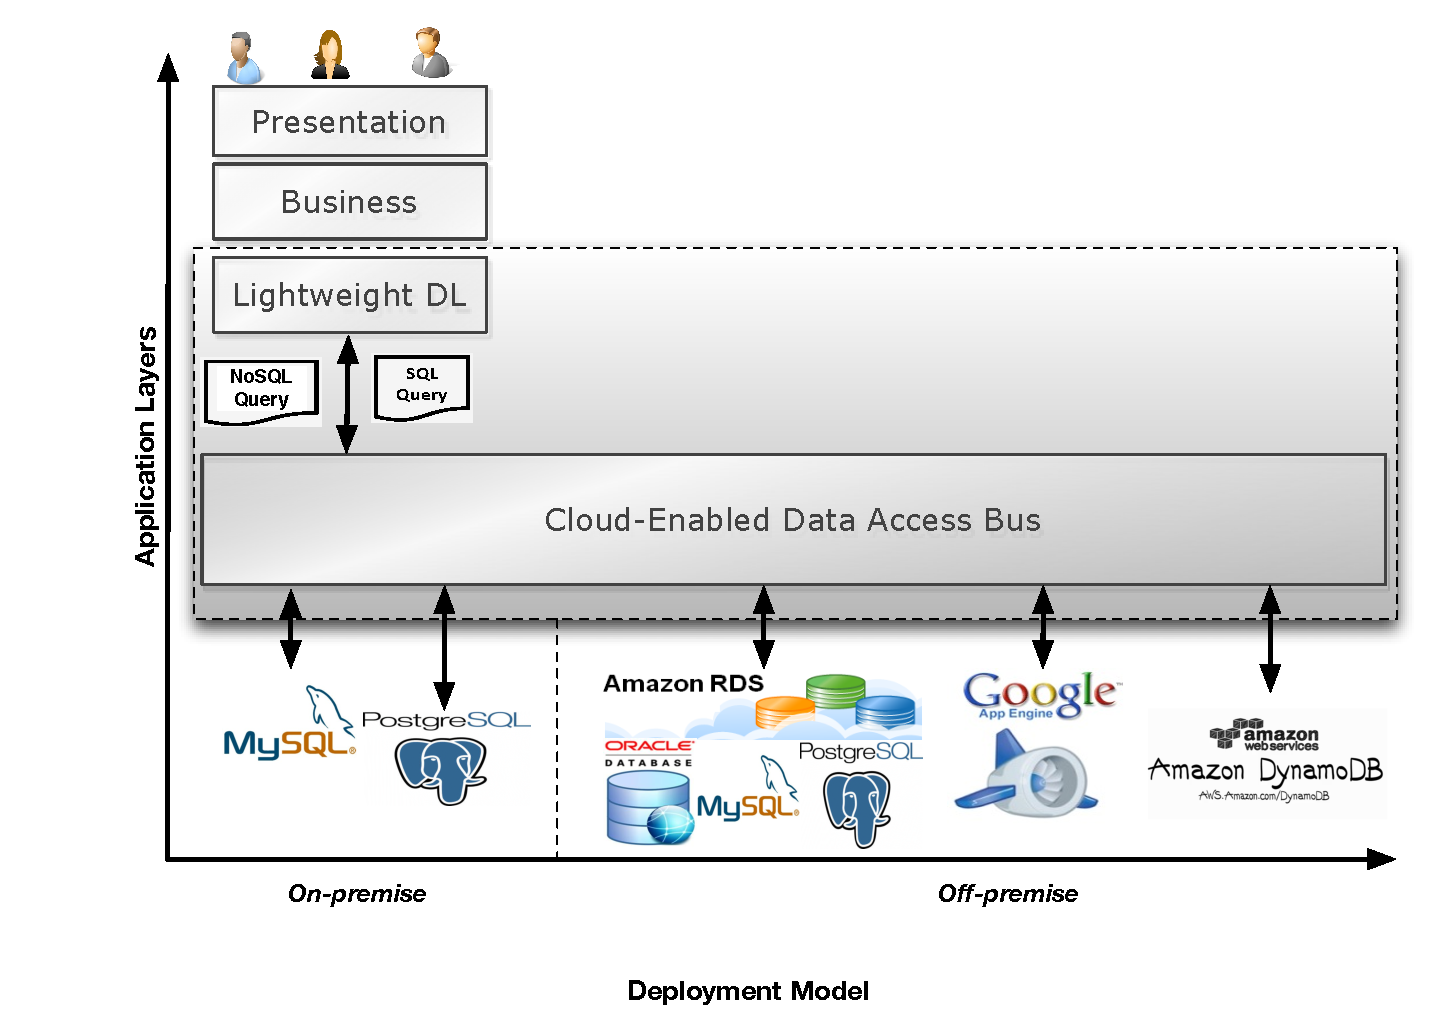
\includegraphics[width=0.925\textwidth, trim=0.0cm 0.0cm 0.0cm 0.0cm, clip]{./gfx/motivationScenario.pdf}
%	\caption[Migration Scenario]{Migration Scenario to be filled }
%	\label{fig:motivationscenario}
%\end{figure}

%As shown in Figure \ref{fig:motivationscenario}, the Cloud-Enabled Data Access bus provides access support between the hosted on-premise, and off-premise application's layers. Its main goal is to provide communication isolation between different applications and users, and maintain the transparency that the DL provided before the migration to the upper layers of the application's architecture. Support must be provided for two different databases types: MySQL and NoSQL databases, and between different providers. A tenant who migrates its data, e.g. to the Google SQL Datastore in Google App Engine, as shown in Figure \ref{fig:motivationscenario}, must be able to access his data with minimum adaptations of the components. Furthermore, storing or retrieving data whose storage is divided into multiple datasources requires a dynamic routing between backend data stores. Compatibility between different SQL and NoSQL databases must be also ensured. However, query and data transformation between different data sources types is out of the scope of this diploma thesis.  


%\FloatBarrier

Der Aufwand bei der Bestimmung der Dokumentähnlichkeit für mehrere Quellen ist in der Regel mit hohem Zeitaufwand verbunden. Vor allem die Bestimmung der Ähnlichkeit in einem Haufen von Daten, die sich entweder im Internet befinden oder in gegebenen Datenspeicher. Hier setzt eine Informationsrückgewinnungslösung an. Diese versucht die Bestimmung der Ähnlichkeit zwischen Dokumente durchzuführen. Dafür gibt es mittlerweile eine Vielzahl an Ansätze. Je mehr die Übereinstimmung sein soll, desto höher wird der Aufwand sein. Darüber hinaus ergibt sich, dass für die Bestimmung der Dokumentähnlichkeit zwei sich gegenseitig gegenüberstehende Herausforderungen beeinflussen, nämlich der Bestimmungsaufwand und den Wunsch Dokumente mit der höchsten Übereinstimmung im gesamten Datensee zu finden.  Da dadurch die Nutzer zufrieden sein können. Außerdem kann es passieren, dass Dokumente nicht unbedingt zutreffen, obwohl die als ähnlich bestimmt wurden. Faktoren wie den Kontext, die Semantik sowie die Bedeutung müssen berücksichtigt werden. Um dieses Problem zu lösen, soll einen bestimmten Ansatz basierend auf Bayessche Statistik ausgewählt werden, der diese Faktoren berücksichtigt.  Die vorliegende Arbeit untersucht auf Bayessche Statistik basierende Ansätze zur Dokumentähnlichkeitsbestimmung.

\section{Zielsetzung}
\label{sec:Zielsetzung}

In the following section we list the definitions and the abbreviations used in this diploma thesis for understanding the description of the work.

\subsection*{Definitions}

\subsection*{List of Abbreviations}

The following list contains abbreviations which are used in this document. 

\begin{acronym}[ApacheODEX]
\acro{ACID}{Atomicity, Consistency, Isolation, Durability}
              \acro{API}{Application Programming Interface}
	\acro{ASP}{Application Service Provider}
	\acro{Axis2}{Apache eXtensible Interaction System v. 2}
	\acro{BC}{Binding Component}
	\acro{BLOB}{Binary Large Object}
		\acro{BPEL}{Business Process Execution Language 2.0}
	\acro{C-CAST CMF}{Project Context Casting (C-CAST) Context-Management Framework}
		\acro{CLI}{Command-line Interface}
	\acro{CLOB}{Character Large Object}
	    \acro{CORBA}{Common Object Request Broker Architecture}
	         \acro{DBaaS}{Database-as-a-Service}
	           \acro{DBMS}{Database Management System}
	             \acro{DBS}{Database System}
	                  \acro{DCOM}{Distributed Component Object Model}
	                      \acro{DCE}{Distributed Computing Environment}
	\acro{EAI}{Enterprise Application Integration}
	\acro{EAR}{Enterprise Archive}
	\acro{EJB}{Enteprise JavaBeans}
	             \acro{EIP}{Enterprise Integration Patterns}
	\acro{ESB}{Enterprise Service Bus}
	        \acro{GAE}{Google App Engine}
	            \acro{HTTP}{Hypertext Transfer Protocol}
	\acro{IaaS}{Infrastructure-as-a-Service}
	\acro{IDE}{Integrated Development Environment}
	\acro{JAR}{Java Archive}
	\acro{Java EE 5}{Java Platform, Enterprise Edition v. 5}
	      \acro{J2EE}{Java 2 Platform, Enterprise Edition}
    \acro{JAX-WS}{Java API for XML-Based Web Services}
    \acro{JAXB}{Java Architecture for XML Binding}
	\acro{JBI}{Java Business Integration}
	\acro{JBIMulti2}{JBI Multi-tenancy Multi-container Support}
	\acro{JDBC}{Java Database Connectivity}
	\acro{JDK}{Java Development Kit}
	\acro{JMS}{Java Message Service}
	\acro{JMX}{Java Management Extensions}
	         \acro{JNDI}{Java Naming and Directory Interface} 
	\acro{JOnAS}{Java Open Application Server}
	\acro{JPA}{Java Persistence API}
	             \acro{JSON}{JavaScript Object Notation}
	\acro{JSF}{JavaServer Faces}
	\acro{JVM}{Java Virtual Machine}
	        \acro{LRU}{Least Recently Used} 
	\acro{MBean}{Managed Bean}
		\acro{MDBS}{Multidatabase System}
		       \acro{MEP}{Message Exchange Patterns}
		             \acro{MOM}{Message-Oriented Middleware}
	\acro{NIST}{National Institute of Standards and Technology}
	       \acro{NM}{Normalized Message}
	        \acro{NMF}{Normalized Message Format}
	\acro{NMR}{Normalized Message Router}
	               \acro{NoSQL}{Not only Structured Query Language}
	\acrodep{OSGi}{Open Services Gateway initiative}
	             \acro{ORDBMS}{Object-relational Database Management System}
	\acro{PaaS}{Platform-as-a-Service}
	\acro{POJO}{Plain Old Java Object}
	        \acro{POM}{Project Object Model}
	\acro{QoS}{Quality of Service}
	             \acro{RDBMS}{Relational Database Management System}
	                    \acro{SA}{Service Assembly}
	\acro{SaaS}{Software-as-a-Service}
    \acro{SE}{Service Engine}
            \acro{SMPP}{Short Message Peer-to-Peer}
            \acro{SNMP}{Simple Network Management Protocols}
	\acro{SOA}{Service-Oriented Architecture}
	\acrodep{SOAP}{Simple Object Access Protocol}
	              \acro{SQL}{Structured Query Language}
	              	          \acro{STaaS}{Storage-as-a-Service}
		                 \acro{SU}{Service Unit}
		\acro{TCP}{Transmission Control Protocol}
		       \acro{URI}{Uniform Resource Identifier}
    \acro{UUID}{Universally Unique Identifier}
    \acro{W3C}{World Wide Web Consortium}
            \acro{WAR}{Web Application Archive} 
    \acro{WS*}{Web Services (Specifications)}\acused{WS*}
    \acro{WSDL}{Web Services Description Language}
    \acro{WSS4J}{Apache Web Services Security for Java}
    \acro{XML}{eXtensible Markup Language}
    \acro{XSD}{XML Schema Definition}
    \acro{XSLT}{Extensible Stylesheet Language Transformation}
             

            

\end{acronym}
\section{Aufbau der Arbeit}
\label{sec:Aufbau der Arbeit}

The remainder of this document is structured as follows:

\begin{itemize}
\item \textbf{Fundamentals, Chapter \ref{chap:fundamentals}:} provides the necessary background on the different concepts, technologies, and prototypes used in this diploma thesis.
\item \textbf{Related Works, Chapter \ref{chap:relatedworks}:} discusses relevant State of the Art and positions our work towards it.  
\item \textbf{Concept and Specification, Chapter \ref{chap:spec}:} functional and non-functional requirements are discussed in this section.
\item \textbf{Design, Chapter \ref{chap:design}:} gives a detailed overview of the differerent component's architecture, and the needed extensions to the already existing ones.
\item \textbf{Implementation, Chapter \ref{chap:implementation}:} the implemented components, as well as the necessary extensions or changes are detailed in this section from the point of view of coding and configuration. 
\item \textbf{Validation and Evaluation, Chapter \ref{chap:validationevaluation}:} in this chapter we test the final prototype based on the scenario described in this document. 
\item \textbf{Outcome and Future Work, Chapter \ref{chap:outcome}:} we provide a conclusion of the developed work and investigate some ideas in which this diploma thesis can be extended.
\end{itemize}
\chapter{Grundlagen, Analyse von Use Cases zur Dokument\"ahnlichkeitsbestimmung }
\label{chap:Grundlagen}

%In this chapter we give an explanation about the technologies and concepts this diploma thesis relies on. We start describing the fundamental concepts and introduce the components and prototypes that form the basis of our work.

\section{Informationsrückgewinnung}
\label{sec:Informationsrückgewinnung}

In the last decades our world has become more and more interconnected. This interconnection added to the increase of the available bandwidth and the change in business models have forced IT Systems to fulfill its demands, leading to its reorganization into a public utility which offers public services, like water, electricity, etc. The \ac{NIST} defines Cloud computing as "a model for enabling ubiquitous, convenient, on-demand network access to a shared pool of configurable computing resources (e.g., networks, servers, storage, applications, and services) that can be rapidly provisioned and released with minimal management effort or service provider interaction"  \cite{NIST2011}. The Cloud computing model is composed of five characteristics:
	\begin{enumerate}
		\item On-demand self-service: a Cloud user consumes the Cloud provider's computing capabilities automatically without the need of human interaction. 
		\item Broad network access: computing capabilities are available via the network and can be accessed using standard mechanisms.
		\item Resource pooling: computing capabilities in the Cloud provider side are virtualized to serve multiple consumers simultaneously using a multi-tenant model. The Cloud consumer generally has no sense of the provided resources.
		\item Rapid Elasticity: computing and storage resources can be dynamically (and in some cases automatically) provisioned and released to respond to the actual consumers' demand.
		\item Measured Service: resources' usage is monitored and measured in a transparent way to the Cloud consumer and provider for control and optimization purposes.
	\end{enumerate}

The control that the Cloud consumer has over the computer resources in a Cloud provider infrastructure is defined in three service models: \term{\ac{SaaS}}, \term{Platform-as-a-Service (\ac{PaaS})} and \term{\ac{IaaS}}. \term{\ac{SaaS}} provides to the Cloud consumer access and usage of Cloud provider's applications running on a Cloud infrastructure. The consumer has no control over the underlying infrastructure where the application he uses is deployed. The customer can only control individual application's configurations during his usage of it. \term{\ac{PaaS}} provides the customer with the needed capabilities to deploy applications which's programming language, required libraries, services and tools are supported by the provider. The consumer has no control over the underlying infrastructure where he deploys the application. \term{\ac{IaaS}} is the model which gives most control to the consumer. Thus, the consumer is able to deploy and run arbitrary software and has the control over operating systems, storage and deployed applications, but has no management or control on the underlaying Cloud infrastructure. 

Although the three service models described above provide both data computation and storage capabilities for the consumer, they do not provide to the customer the possibility to directly and uniquely purchase access of storage services. In this diploma thesis we concentrate in two concrete models: \term{\ac{DBaaS}} and \term{\ac{STaaS}}. Cloud storage providers target a selected number of consumers, who process their data on-premise, but do not  want to cover the expenses of a local database system, or a backup system, among others. The Cloud storage model alleviates the need in organizations to invest in database hardware and software, to deal with software upgrades, and to maintain a professional team for its support and maintenance \cite{dbaasIyer}.  \ac{DBaaS} and \ac{STaaS} can be considered quite similar, except for one of their main distinction characteristics: their access interface. The former is the most robust data solution offered as a service, as it offers a full-blown database functionality. It can be accessed via the most common database protocols, such us MySQL, Oracle, etc, or by REST interfaces supporting \ac{SQL}. Examples of this model are Amazon RDS \cite{amazonrds} and Oracle Cloud \cite{oraclecloud}. On the other hand, the latter provides REST, \ac{SOAP} over \ac{HTTP}, or Web-based interfaces in order to perform the operations over the stored data \cite{cloudstorageWU}. Examples of this model are Amazon Dynamo \cite{amazondynamodb} , Google App Engine Datastore \cite{googleappdatastore}, and Dropbox \cite{dropbox}.

\ac{NIST} defines four deployment models in Cloud computing. A private Cloud consists in a Cloud infrastructure which is provisioned exclusively for one organization and used by the members conforming the organization. It is comparable to processing facilities that are enhanced with the Cloud computing characteristics. A community Cloud is a Cloud infrastructure where its use is limited to organizations which share the same requirements. A public Cloud infrastructure can be accessed and used by the public. It is usually offered by Cloud service providers that sell Cloud services made for general public or enterprises. Some of the Cloud consumers may process and store information which requires more control over the infrastructure in which is located, or consume public Cloud computing resources during peak loads in their private Cloud infrastructure. The hybrid Cloud model combines two or more deployment models described above and the combination remains as a unique entity.  

Cloud computing and \ac{SOA} are related styles at an architectural, solution and service level, according to IBM \cite{IBM2011}. Cloud providers expose their Cloud infrastructure as services as part of a \ac{SOA} solutions and the communication between Clouds in the Hybrid Cloud model described above can be compared to a SOA communication solution between enterprises. Cloud services are services that can be accessed by the Cloud consumers through the network. Therefore, we can deduce that the SOA model can be applied in the Cloud computing approach. As the \ac{ESB} is the central piece of \ac{SOA}, the need of the \ac{ESB} in a Cloud computing infrastructure as an integration middleware for the Cloud services is essential. 
\section{Grundlagen der Bayesschen Statistik}
\label{sec:BayesscheStatistik}  

%Weerawarana et al. define SOA as an specific architectural style that is concerned with loose coupling and dynamic binding between services \cite{Weera2005}.

%In the last years communication between external components whose functionalities are exposed as services has been a hard task when there was not previous agreement on message protocols, data types and encoding, and used middleware technology. Due to the economic and technological growth needed, enterprises had to adapt the \ac{SOA} paradigm in their existing IT Infrastructure. \ac{SOA} provides the needed flexibility by building an architectural style with the following benefits: loose coupling, interoperability, efficiency, and standardization. The W3C group defines SOA as a form of distributed system architecture that is typically characterized by the following properties \cite{w3csoa}:
%	\begin{itemize}
%		\item Logical view: the service's functionality is exposed, but not its internal logic.
%		\item Message orientation: the internal structure of an agent is abstracted.
%		\item Description orientation: a service is described by machine-processable meta data.
%		\item Granularity: services tend to use a small number of operations with relatively large and complex messages.
%		\item Network orientation: Services tend to be oriented toward use over a network.
%		\item Platform neutral: Messages are sent in a platform-neutral, standardized format delivered through the interfaces.
%	\end{itemize}

%\ac{SOA} defines three main roles: requester, provider and broker and the four main operations: publish, find, bind, and invoke. The service provider provides access to services, creates a description of a service and publishes it to the service broker. The service requestor discovers a service by searching through the service descriptions located in the service broker. When the service which best fits to his needs is found, the discovering facility provides the concrete service endpoint and the consumer is responsible for binding to it.  With this information, the requestor can then bind to the concrete service and finally execute a business activity \cite{Weera2005}. The service broker provides support for service registration and binding. 

%The main component in a \ac{SOA} is the \ac{ESB}. The functionalities provided by a service bus can simplify the process (publication, discovery, binding, and invocation) and make it more transparent to provide an ease-to-use experience for a Web service based implementation of \ac{SOA} \cite{Weera2005}. Chappel defines its function as an intermediate connection provisioning of service providers with service consumers and thereby ensure decoupling of theses \cite{Chapp2004}. 

\subsection{Definition und Hintergrund}
\subsection{Anwendungsgebiete und Nutzen}
\subsection{Modelle, Parameter und Überzeugungen}
\subsection{Die Wahrscheinlichkeit}
\subsection{Der Satz von Bayes}
%The flow of data and information is a key for driving business decisions in IT organizations \cite{Chapp2004}. Furthermore, the interaction between loosely coupled components within an organization or with third party organizations requires distributed systems mechanisms which provide communication support for different protocols, and reliability. SOA has fulfilled this main requirement by providing an integration environment with minimal (or any) integration efforts. 

%The \ac{ESB} is the central component in \ac{SOA}. It provides a loosely coupled, event-driven \ac{SOA} with a highly distributed universe of named routing destinations across a multi-protocol message bus \cite{Chapp2004}. An \ac{ESB} provides an abstract decoupling between connected applications by creating logical endpoints which are exposed as services and conform a multi-protocol environment, where routing and data transformation are transparent to the service connected to it. Furthermore, when using an \ac{ESB}, in the first place, services are configured rather than coded, demanding minimal adaptation, implementation and maintenance efforts. The programmer just has to implement the binding to the logical endpoint exposed as a service. In the second place, \ac{ESB} routing is based on a reliable messaging router. Applications don't need to include message system-failure forwarding mechanisms, to know which data formats are needed in the consumed services, or to care about future changes in applications or services the applications interact with. An \ac{ESB} hides the complexity of orchestration between services in business processes. 

%Chappel defines the combination of loosely coupled interfaces and asynchronous interactions as a key concept of the bus terminology  \cite{Chapp2004}. A user of the bus can access every service registered in the bus. For this purpose, it implements the \ac{SOA} operations in order to make them transparent to the user who can therefore focus on: plugging to the bus and posting and receiving data from the bus. Furthermore, the \ac{ESB} can form the core of a pervasive grid \cite{Chapp2004}. Services supported by an organization can be organized between the \ac{ESB}s conforming the grid, as well as its access between the organizational departments, and services provided to third party organizations. 

%\begin{figure}[htb]
%	\centering
%		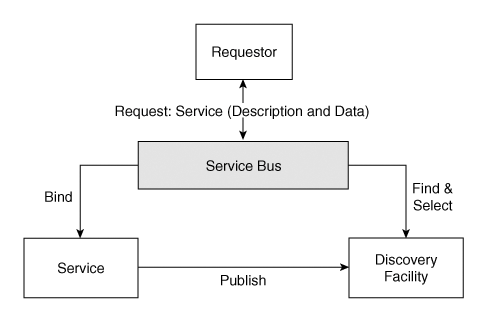
\includegraphics[clip, scale=0.7]{./gfx/servicebus.png}
%	\caption[The Role of the service bus in SOA]{The Role of the service bus in \ac{SOA} \cite{Weera2005} }
%	\label{fig:servicebus}
%\end{figure}

%(see Figure \ref{fig:servicebus})

%When receiving a service description (\ac{WSDL}) and data from the service requester, the \ac{ESB} is responsible for selecting the service which best fits to the description requirements, for binding the service requester with the backend service through a route created between the logical endpoints and for making the necessary data transformations to enable the communication between the parts.

%As the \ac{ESB} is the central component in \ac{SOA}, and established as integration middleware for services, in this diploma thesis we focus on the required modifications and extensions in the open-source \ac{ESB} Apache ServiceMix 4.3 to provide transparent communication support between the applications and its data located in on-premise databases, or migrated to off-premise data stores. 

%\FloatBarrier
\section{Analyse von Use Cases für die Dokumentähnlichkeitsbestimmung}
\label{sec:AnalyseUse}   

One of the main decision variables for utilizing a Cloud computing environment are capital expenditures. The main goal of a Cloud consumer is to minimize its business costs when migrating to the Cloud. According to Chong, a \ac{SaaS} solution benefits a Cloud customer with the following advantages \cite{ChongB2006}:

	\begin{itemize}
		\item The Cloud consumer does not directly purchase a software license, but a subscription to the software offered as a service by the Cloud infrastructure. 
		\item More than half of the IT investments of a company are made in infrastructure and its maintenance. In a \ac{SaaS} solution this responsibilities are mainly externalized to the Cloud provider.   
		\item A Cloud computing environment is based on the utilization of its resources simultaneously by a large number of Cloud consumers. For example, a Cloud provider that offers a centrally-hosted software service to a large number of customers can serve all of them in a consolidated environment and lower the customer software subscription costs while maintaining or lowering the provider's infrastructure, administration and maintenance costs. 
		\item The cost leverage in the software utilization allows the Cloud providers to focus not only on big enterprises capable of large IT budgets, but also on the small business that need access to IT solutions. 
	\end{itemize} 

Multi-tenancy in a \ac{SaaS} environment allows the Cloud providers to lower the cost per customer by optimizing the resources usage in the Cloud infrastructure. The software serves multiple tenants concurrently, who share the same code base and data storage systems. Chong and Carraro \cite{ChongB2006} define a well designed \ac{SaaS} application as scalable, multi-tenant-efficient and configurable. With this design patterns, the \ac{SaaS} model enables the provider to \term{catch the long tail}. Business softwares are becoming more complex and tend to demand an individual customer support and an increase of the computing and storage resources in the infrastructure. This fact leads to an increase in the infrastructure investment and maintenance costs. However, if the previous requirements are eliminated and the provider's infrastructure is scaled to combine and centralize customers' hardware and services requirements, the price reduction limit can be decreased and, in effect, allow a wide range of consumers to be able to access this services.

The reasons discussed above are also applicable in the \ac{DBaaS} and \ac{STaaS} models. Storage and retrieval of data involve high maintenance and management costs. The data management cost is estimated to be between 5 to 10 times higher than the data gain cost \cite{multishares2011}. Furthermore, storing data on-premise does not only require storing and retrieving data, but also requires dealing with disaster recovery, \ac{DBMS}, capacity planning, etc. Most of the organizations prefer to lead their investments to their local business applications rather than becoming a data management company \cite{multishares2011}. Cloud storage providers offer a pay-per-use storage model, e.g. based on storage capacity or based on number of connections to the storage system, and ensure that the stored data will persist over time and its access through the network. However, security and confidentiality are the main constraints when moving private data to a shared public infrastructure. 

\begin{figure}[htb]
	\centering
		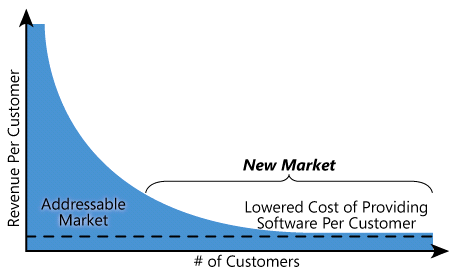
\includegraphics[clip, scale=0.5]{./gfx/longtail.png}
	\caption[Multi-tenancy and Long Tail]{New market opened by lower cost of SaaS \cite{ChongB2006}}
	\label{fig:longtail}
\end{figure}

In the Figure \ref{fig:longtail} the economics of scaling up to a high number of customers while reducing the software price is analyzed. Cloud providers have reached a new market formed by small or medium businesses without enough budget for building an on-premise IT infrastructure.

Multi-tenancy refers to the sharing of the whole technological stack (hardware, operating system, middleware, and application instances) at the same time by different tenants and their corresponding users \cite{EnablingMT}. Andrikopoulos et al. identify two fundamental aspects in multi-tenant awareness: communication, and administration and management \cite{andrikopoulos2013}. The former involves isolated message exchanges between tenants and the latter allows tenants individual configuration and management of their communication endpoints. Utilizing an \ac{ESB} as the central piece of communication middleware between applications in a \ac{PaaS} environment forces it to ensure multi-tenancy at both communication, and administration and management, as mentioned before. The multi-tenancy support modifications made in the open-source ServiceMix 4.3 are the results of \cite{Essl2011}, \cite{Muhler2012}, and \cite{gomez2012}. In this diploma thesis we reuse and extend those results in oder to provide multi-tenant transparent Cloud data access in the Cloud through the \ac{ESB}, when the application's data is migrated and accessed through the \ac{ESB} in a Cloud infrastructure.

The migration of an application's stack to the Cloud can be done at different levels of the application's stack: Presentation Layer, Business Layer, and Data Access Layer. The Replacements of Components with Cloud offerings migration type is the least invasive type of migration \cite{andrikopoulos2013}. In this diploma thesis we focus on this type of migration, concretely when the used Cloud offering is the database system. Migration of the data can be either seen as the migration of the Data Layer (Data Access Layer and Database Layer) or of the whole application \cite{andrikopoulos2013}. Migration of the Data Layer to the Cloud means migrating the both data management and data access to the Cloud, while maintaining its transparency to the application's Business Layer. 

In a Cloud infrastructure where Cloud storage is offered, Feresten identifies four main tenant requirements: security, performance, data protection and availability, and data management \cite{feresten2010}. Multi-tenancy in a storage system can be achieved by aggregating tenant-aware meta-data to the tenant's data (see Figure \ref{fig:virtualstoragecontainer}), or by physical storage partitioning, but this is not sufficient when fulfilling the data management, and the flexibility requirement. Tenants must have independent access and management, as if they accessed their own data storage systems. For this purpose, storage vendors have introduced the concept of \term{virtual storage container}, a tenant-aware management domain which grants all (or most of) the database management operations over the storage container, as described in Figure \ref{fig:virtualstoragecontainer}.

\begin{figure}[htb]
	\centering
		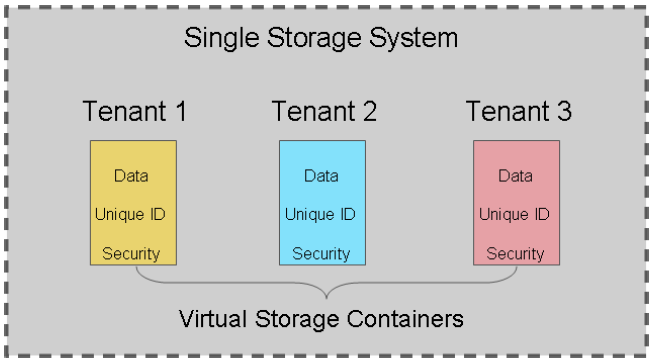
\includegraphics[clip, scale=0.4]{./gfx/virtualstoragecontainer.png}
	\caption[Virtual Storage Container]{Attributes of a Virtual Storage Container \cite{feresten2010}}
	\label{fig:virtualstoragecontainer}
\end{figure}

In this diploma thesis we must take into account the different approaches that most of the Cloud storage vendors have taken into account, in order to provide the tenant transparent access through the \ac{ESB} to his virtual storage container in one or more Cloud infrastructures.

\subsection{Finden von Dokumenten mit ähnlichen Inhalten(Duplikaten Findung)}
\subsection{Verwendung von a priori Wissen}
\subsection{Systemübergreifende „Fremdschlüssel"}
\subsection{Profil Matching}
\subsection{Email Klassifikation (Spamfilter)}
\input{fundamentals/AnalyseAnsätze}

\chapter{Die Informationsrückgewinnung-Middleware-Lösung}
\label{chap:BD4B}

\section{Vorstellung}
\label{sec:VorstellungBD4B}  

In this section we describe the \ac{JBI} \ac{BC}s shipped in the ServiceMix-mt prototype this diploma thesis focuses on, and the transport protocols they support. 



ServiceMix provides \ac{HTTP} communication support in its \ac{HTTP} \ac{JBI} \ac{BC}. Its \ac{HTTP} consumer and provider endpoints are built on the \ac{HTTP} Jetty 6 server and Jakarta Commons \ac{HTTP} Client respectively, providing support for both REST and SOAP over HTTP 1.1 and 1.2 requests.

The original \ac{HTTP} \ac{BC} is extended in the ServiceMix-mt prototype to provide multi-tenant support in \cite{Muhler2012} and \cite{gomez2012}. Muhler provides an internal dynamic creation of tenant-aware endpoints in the \ac{BC}, by injecting tenant context in the \ac{JBI} endpoint's URLs \cite{Muhler2012}. Gomez provides a \ac{NMF} with tenant context information in its properties for routing in the \ac{NMR} \cite{gomez2012}. However, in this diploma thesis we must not only provide tenant isolation at the tenant level, but also isolation at the user level. We discuss this requirement in detail in Chapters \ref{chap:spec} and \ref{chap:design}.

\begin{figure}[htb]
	\centering
		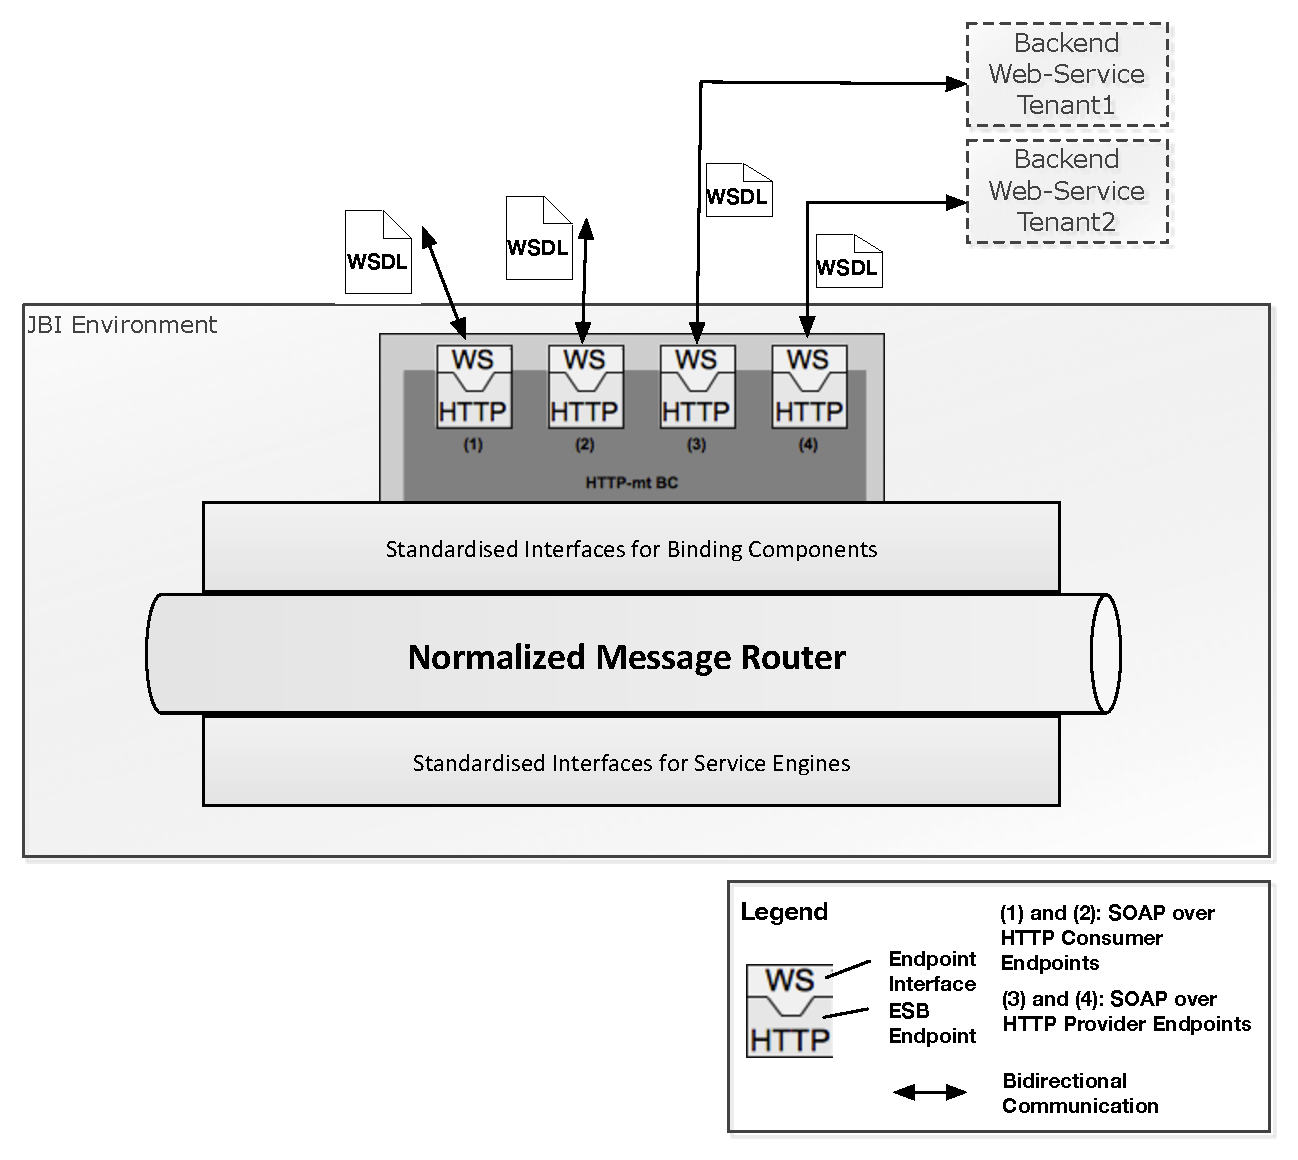
\includegraphics[clip, scale=0.3]{./gfx/httpmtbc.pdf}
	\caption[Multi-tenant HTTP Binding Component]{Multi-tenant HTTP Binding Component \cite{gomez2012}. }
	\label{fig:httpmt}
\end{figure}

As seen in Figure \ref{fig:httpmt}, the multi-tenant \ac{HTTP} \ac{BC} is mainly used in ServiceMix-mt to support the \ac{SOAP} over \ac{HTTP} communication protocol by exposing a Web service in the tenant-aware consumer endpoint and consuming an external Web service in the provider endpoint. \ac{SOAP} defines an \ac{XML} message format  which is sent over the network and a set of rules for processing the \ac{SOAP} message in the different \ac{SOAP} nodes which build the message path between two endpoints \cite{Weera2005}. A \ac{SOAP} message is a composition of three main elements: a SOAP envelope, header, and body. A SOAP envelope may contain zero or more headers and one body. The header may contain processing or authentication data for the ultimate receiver or for the intermediate nodes through the message is routed. The message payload or business data is included in the SOAP body. SOAP is used as a message framework for accessing Web services in loosely coupled infrastructures \cite{Weera2005}. The Web service consumer specifies the functionality to invoke in the SOAP body. If the Web service functionality has a request-response \ac{MEP}, a SOAP message is used to send the response data when the corresponding operation has been executed successfully or the error data in case an error occurred during execution.

Most of the Cloud storage providers provide an \ac{HTTP} interface to the tenants for data management, retrieval, and storage. In this diploma thesis we extend this \ac{JBI} \ac{BC} in order to provide the tenant a transparent access to his \ac{NoSQL} Cloud data stores.

\FloatBarrier

\section{Anforderungen}
\label{sec:AnforderungenBD4B}

The \ac{JNDI} defines a framework for deployment support in a \ac{JVM} of downloaded or extended applications known as \term{bundles}. This framework requires OSGi-friendly devices a minimum system's resources usage by providing dynamic code-loading and \term{bundle} lifecycle management. An \ac{OSGi} \term{bundle} is the packaging of a group of Java classes and required and provided capabilities' meta-data as a JAR file for providing functionality to end users. \ac{OSGi} \term{bundles} can be downloaded, extended and installed remotely or locally in the platform when needed without the need of system reboot. Installation and update of bundles during their lifecycle are also managed by the framework, which uses a service registration for selection, update notifications, or registry of new service objects offered by a deployed bundle. This feature is the main key for connecting bundles whose's services require during runtime capabilities provided by another bundles. The framework defines a bundle's requirement capability as a dependency.      

The \ac{OSGi} framework defines 5 different layers and a bundle's lifecycle \cite{OSGi2011}. An optional Security Layer provides the infrastructure for deploying and managing applications which must be controlled during runtime. The Module Layer lists the rules for package sharing between the deployed bundles. The lifecycle of a bundle can be modified during runtime through an API provided in the lifecycle layer. The main operations implemented are install, update, start, stop or uninstall. 

\subsection{Funktionelle Anforderungen}
\subsection{Nicht funktionelle Anforderungen}
\subsection{Plattformanforderungen}
\subsection{Komponentenanforderungen}
\subsection{Anforderungen an dem Ähnlichkeitsalgorithmus}
\section{High-Level Architektur}
\label{sec:HighLevelArchitektur}  

A multi-tenant management system must fulfill several requirements, such as data and performance isolation between tenants and users, authentication, specification of different user roles, resources usage monitoring, etc. In a \ac{JBI} environment, endpoint and routing configurations files are packed in \ac{SU}s, and the latter in \ac{SA}s for deployment. However, there is a lack of user-specific data during deployment. Muhler solves this problem in JBIMulti2 by injecting tenant context in the \ac{SA} packages, making them tenant-aware \cite{Muhler2012}. 

\begin{figure}[htb]
	\centering
		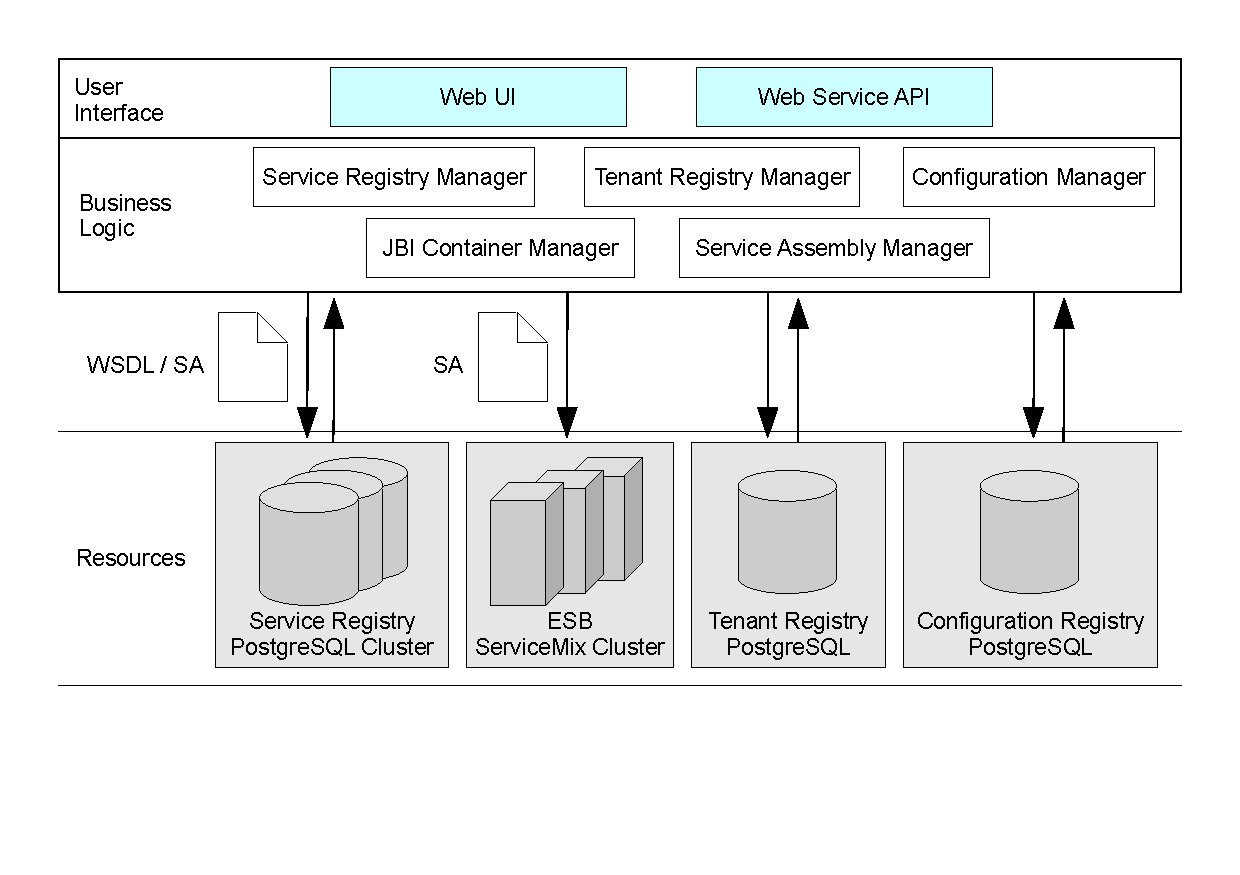
\includegraphics[clip, scale=0.5]{./gfx/systemoverview_jbimulti2.pdf}
	\caption[JBIMulti2 System Overview]{JBIMulti2 System Overview \cite{Muhler2012}} 
	\label{fig:jbimulti2}
\end{figure}

The architecture of the JBIMulti2 system is represented in Figure \ref{fig:jbimulti2}. We can distinguish two main parts in the system: business logic and resources. JBIMulti2 uses three registries for storing configuration and management data. When a tenant (or a tenant user) is registered, an unique identification number is given to them and stored in the Tenant Registry. Both Tenant Registry and Service Registry are designed for storing data of more than one deployed application. The former for storing tenant information and the latter for providing a dynamic service discovery functionality between the different applications accessed through the \ac{ESB}. The Configuration Registry is the key of the tenant isolation requirement of the system. Each of the stored tables are indexed by the tenant id  and user id value. In this thesis we need tenant information during runtime. We reuse and extend the databases schemas produced by Muhler, specifically the Service Registry.

The system provides a user interface for accessing the application's business logic. Through the business logic, the management of tenants can be done by the system administrator or the management of tenant's users can be done by the tenants. Furthermore, when deploying the different tenant's endpoint configurations packed in \ac{SA}s, the system first makes modifications in the zip file for adding tenant context information and then communicates with the Apache ServiceMix instance by using a \ac{JMS} Topic to which all the ServiceMix instances are subscribed to. The \ac{JMS} management service in ServiceMix deploys the received \ac{SA} injected in the received \ac{JMS} message using the administration functionalities provided in ServiceMix. The communication between the business layer and the ServiceMix instance is unidirectional. When successful deployment, the endpoint is reachable by the tenant. When an error occur during deployment, an unprocessed management message is posted in a dead letter queue.

JBIMulti2 requires the previous installation of components, e.g. JOnAS server, PostgreSQL, etc. The initialization of the application is described in both Chapter \ref{chap:validationevaluation} and in the JBIMulti2 setup document \cite{JBIMulti2Man}.

%\clearpage 

%In this chapter we provide a general overview on the different approaches that are taken into account in order to provide a reliable, secure, and transparent communication between on-premise application's layers and off-premise Cloud data stores. Furthermore, we discuss about the needed adaptations different authors specify that the on-premise application's layers must address when migrating their underlying layers to a Cloud infrastructure. We compare it to the ones we transparently support in our approach, and the ones the user should consider. We finally mention the improvements we need to perform to the original prototype ServiceMix-mt, and continue our discussion dividing it into the two main \ac{DBMS} available nowadays in the market: \ac{SQL} and \ac{NoSQL} databases.

%% non functional data layer patterns paper: make a big emphasis on the proxy approach. It is quite similar to our approach, because it allows horizontal scalability between different target data sources, but there is no need of abstracting the proxy from the database layer. esb's are horizontally scalable and can form a esb cluster, as described in the esb part in fundamentals. we can have in our approach a bottleneck when using one instance of the esb. furthermore, their proxy approach assumes that the database layer is in the private cloud, while in ours the database layer can reside either on or off premise.
%A migration process of the Database Layer of an application to the Cloud may pop up several incompatibilities with the new hosting environment, which need to be addressed prior to the migration decision. Strauch et al. aim to address such incompatibilities by defining a set of \term{Cloud Data Patterns}, which target finding a solution for a challenge related to the data layer of an application in the Cloud for a specific context \cite{strauchABKL2012}. Incompatibilities a user may find when migrating the application's data layer can be on the level of the schema representation, supported set of queries or query language, communication protocol, security, etc. Strauch et al. focus mainly in two non-functional aspects: enabling data store scalability and ensuring data confidentiality \cite{strauchABKL2012}. 

%The former deals with maintaining the quality of service levels when the workload increases, for both write and read operations. There are two scalability mechanisms when dealing with data: vertical and horizontal scalability. A vertical scalable system can be obtained by introducing more powerful hardware, or moving to a more powerful database system, while a horizontal scalable system deals with splitting data into groups which are stored in different partitions or different database systems, also known as \term{sharding}. Due to the absence of support for accessing a \term{sharded database} between different database systems, the concepts of a database proxy and sharding-based router are introduced. In this first approach, a proxy component is locally added below each data access layer \cite{strauchABKL2012}. A proxy below each data access layer instead of a common proxy on top of the database layer dismisses a common point of failure when accessing the data. In the second approach, a local sharding-based router is added below each of the data access layer. A sharded-based router contains the needed knowledge about the location of the \term{sharded databases}. In our approach, we don't only partially follow both of the concepts, but integrate them in a single component. We consider a sharded-based router as a proxy with routing capabilities. Therefore, as it is discussed in Chapter \ref{chap:design}, enhancing an \ac{ESB} with the required \term{sharded databases} knowledge and with standardized communication protocols, it allows us to utilize it as a sharded-based router, and as a proxy. Furthermore, the single point of failure avoidance can be ensured by increasing the number of \ac{ESB} instances and balancing the load between them. As discussed before, we do not fully comply with this approach. The development of a proxy or sharded-based router component below each data access layer forces each application to deploy at least one proxy or sharded-router instance in their system. In our approach we propose the utilization of our prototype as a shared transparent Cloud data access layer by connecting to a data access endpoint which supports a specific \ac{DBMS} multi-tenant aware communication protocol (e.g. MySQL or PostgreSQL). For this purpose, we propose the concept of a lightweight Data Layer, where the adaptations to its sublayers are minimized, e.g. modification of data access host, port, etc. The data access endpoint acts as a database protocol-aware proxy, forwarding the requests to the \ac{NMR} of the \ac{ESB}. We enhance the Myosotis Tungsten Connector and provide access control, caching functionality, and full integration in the \ac{ESB} \ac{OSGi} container, and with the \ac{NMR} \cite{tungstenwiki}.

%% Data confidentiality between the on premise app layers and the migration layers and how can we still ensure data confidentiality: mention the 5 patterns that are in steve's article. Mention that this article gives a deep focus on security patterns rather than technical information regarding the router between the data stores. we do not implement automatic data filtering for confidentiality. the user is the one who decides which data goes off premise and which data stays in premise. we provide support for off premise and on the on premise data. however, this can be reached in our esb but requires user customization, in order to be able to filter data per user and to route it to the appropriate data store.

%Ensuring data confidentiality is presented in \cite{strauch2012}. Their work deals with critical data management between on-premise and off-premise data stores, and categorizes data into different confidentiality levels to prevent data disclosures. The former is achieved by aggregating information which categorizes data into different categories and confidentiality levels. The latter deals with keeping confidential data on-premise. With data filtering, pseudonymization, and anonymization, data is either prevented from being externally routed, or secured when routed to a public Cloud \cite{strauch2012}. The pseudonymization technique provides to the exterior a masked version of the data while maintaining its relation with the original data, and the anonymization provides to the exterior a reduced version of the data. In this diploma thesis' approach, we assume that the application's owner has decided on which data should be and cannot be migrated, and that the business layer is hosted on-premise. Therefore, there is no data processing in a public Cloud environment. Our final prototype provides confidentiality between different tenants of the system by injecting tenant information  in our messages and providing tenant-aware routing, and different multi-tenant aware endpoints. We do not need to provide support for pseudonymization or anonymization techniques, in contrast to \cite{strauch2012}.

%% table of what do i have to do when migrating app or app components to the cloud. this is from the book chapter of vasilios and steve. comment here what ive written in the comments
%Replacement of components which build an application with Cloud offerings leads the developers to face an application's adaptation process. For example, migrating a local database to a private Cloud or to a public Cloud, or sharding a database between on-premise and off-premise data stores forming a single data store system, can not be accessible without adapting the non-migrated application's layers to the new storage system. Andrikopoulos et al. identify the needed adaptations actions when migrating a data layer to the Cloud \cite{andrikopoulos2013}: address reconfiguration, patterns realization, incompatibilities resolution, query transformation, and interaction with data store allowance. Our main goal in our final prototype is to minimize the number of adaptations the user must perform when migrating application's data to a Cloud data store. The adaptations of the \ac{ESB} must encompass the described adaptations in a transparent way to the user, in order to internally support in our prototype compatibility between the application and the different data stores, and lower the adaptation operations number at the application's side, e.g. only address reconfiguration. 

%% speak a little bit about federated databases
%% have taken notes in the paper. the main thing to say here is the main difference between a federated database system and our approach. Our approach works more or less than a federated database system, but more like a federated server, where transparent access to backend datasources is provided. joins are out of the scope of the thesis. indicate that one main component in a federated dbs is the transformer, in our case between sql databases, and between nosql databases, but this is out of scope of this thesis. 
%% mediator in page 37 of the book principles of distributed database systems
%Federated Database Systems are a type of \ac{MDBS} that allow accessing and storing data which is stored in different and noncontiguous databases through a single interface. Sheth and Larson define them as a collection of cooperating but autonomous component database systems, which can be integrated to various degrees, and can be accessed by a software which controls and coordinates the manipulation of the database systems which conforming the federated database system. This distributed database model allows users to access and store data among different database systems, which can be located in different continents, without dealing with multiple connections to the different database systems, query and data transformation, address adaptation, etc. \ac{MDBS} are accessed through a single endpoint which provides a single logical view of the \ac{MDBS}, and users can access the different \ac{DBMS} which form the \ac{MDBS} (see Figure \ref{fig:multidatabasesystem}). 

%\begin{figure}[htb]
%	\centering
%		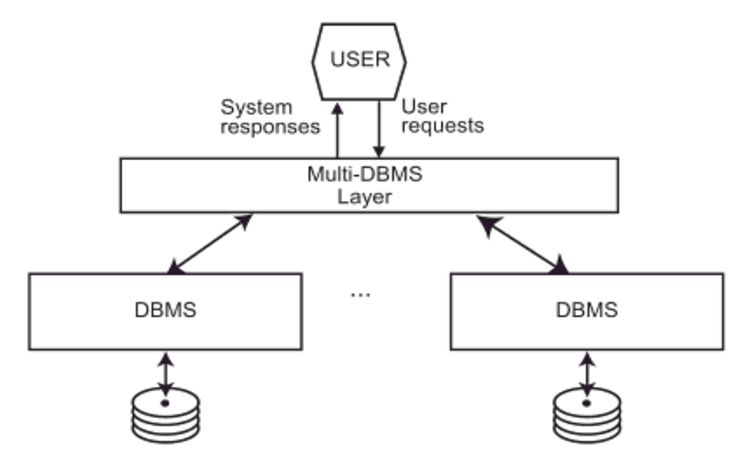
\includegraphics[clip, scale=0.6]{./gfx/multidatabasesystem.pdf}
%	\caption[Multidatabase System Components]{Components in a multidatabase %system \cite{ddbsozsu}}
%	\label{fig:multidatabasesystem}
%\end{figure}

%A popular implementation architecture for a \ac{MDBS} is the mediator/wrapper approach \cite{ddbsozsu}. Mediators exploits knowledge to create information for upper layers, while wrappers provide mapping between different views, e.g. relational vs. object-oriented views. We can consider our approach as a \ac{MDBS} with some modifications and less functionalities. In the first place, using the \ac{ESB} as a single entrance point to the data system while managing different backend autonomous Cloud or traditional data stores comply with the main concept of a \ac{MDBS}. Furthermore, Cloud data store providers may implement the same distributed database model, whereby we could find two logical levels for accessing the physical data. However, we do not accurately follow the mediator/wrapper approach. In our approach we exploit data provided by the tenant during the migration decision and process, by providing an interface to register the backend data store/s information in our system, for future routing purposes. Furthermore, compatibility information is registered in order to apply the needed query or data transformation between data stores. However, the transformation is out of the scope of this diploma thesis, and the support of table joins between databases located in different Cloud data stores are out of scope as well.
%%tenant isolation approach in muhler versus tenant and user isolation approach in this work. explain the granularity of tenant and users, one tenant may want to migrate his database to a data store, but in this case one database can have one or more users. it is not like in muhlers approach where tenants are considered applications accessing the esb. 

%As described in the previous chapter, multi-tenancy is one of the main requirements in a Cloud environment. Muhler, Essl, and Gomez provide an extended version of ServiceMix 4.3, which supports multi-tenancy at two different levels: communication, and administration and management \cite{Muhler2012}, \cite{Essl2011}, \cite{gomez2012}. However, their prototype supports tenant isolation at the level of tenants. A \ac{DBMS}, e.g. MySQL, by default provides access to one default user and supports multiple users creation \cite{mysqlmanual}. Therefore, in our approach we must not only consider isolation at the tenant level, but also at the user level. We assume that the tenant is the default user which migrates his data store to a Cloud environment, but the migrated data store may contain one or more users. In our prototype we ensure tenant and user isolation at both communication, and administration and management levels.

%% caching mechanism used in our approach, explaining the two levels of caching that we use. compare it to the actual mysql proxy and to the databases architectures in the cloudcomputingdatabaseapps paper, say that caching is not discussed in their approach. caching applies for both mysql and nosql. drivers provided by the different vendors do not provide caching functionality. caching functionality must be trated in the application or in the server. caching is good not only for performance, but also to give the possibility to reduce costs in the tenants data stores in the cloud. most of the providers dont only charge per storage size, but also per calls to their api
%%mention the paper
%% put examples on amazon pricing : Micro DB Instance	$0.025 Small DB Instance	$0.090 Medium DB Instance	$0.180 Large DB Instance	$0.365 Extra Large DB Instance	$0.730 this are prices of usage per hour
%% amazon dynamo db: Write Throughput: $0.01 per hour for every 10 units of Write Capacity - Read Throughput: $0.01 per hour for every 50 units of Read Capacity
%% google cloud storage: (per 1,000 requests/month) PUT, POST, GET bucket**, GET service** Requests $0.01 - GET, HEAD Requests (per 10,000 requests/month) $0.01 - DELETE Requests free
%Over the past decades, caching has become the key technology in bridging the performance gap across memory hierarchies via temporal or spatial localities; in particular, the effect is prominent in disk storage systems \cite{cashing2012}. Han et al. investigate how cost efficiency in a Cloud environment can be achieved, specially in applications which require a high I/O activities number, and present a CaaS (cache-as-a-service) model. Cloud providers offering data storage solutions present pricing models based on the storage size, usage per time, or number of requests. Amazon RDS costs \$0.025 per hour for a Micro DB Instance usage  \cite{amazonrds}, while Amazon DynamoDB \$0.01 per hour for every 50 units of read capacity \cite{amazondynamodb}, and Google Cloud Storage \$0.01 per 1000 PUT, POST, GET requests per month \cite{googlecloudstorage}. An I/O-intensive application whose database is hosted in the Cloud may produce a significant economic cost. The cost of continuously retrieving data from the Cloud data store, when existing temporal proximity between the data accessed, can be considered unnecessary, and reducible. Furthermore, the application's overall performance can be reduced due to the network latency and, in the scope of this work, the use of an \ac{ESB} to access the Cloud data store. In this diploma thesis we do not provide cashing as a service, but include cashing support to the sharded-based router pattern described in \cite{strauchABKL2012}. Uralov enhaces ServiceMix-mt with cashing support for dynamic discovery and selection of Cloud data hosting solutions \cite{Uralov2012}. However, we must adapt and extend it due to the lack of support of functionalities we require and the lack of full \ac{OSGi} compliance. 

 
\chapter{Auswahl von Ansätzen zur Dokumentähnlichkeitsbestimmung in der Information-Retrieval-Middleware-Lösung }
\label{chap:AuswahlAnsätzen}

In this chapter we first provide an overview of the system and its components which provide support for accessing on-premise and off-premise Cloud data stores after migrating the data to the Cloud. In the second part of this chapter we specify the functional and non-functional requirement the system must fulfill, and provide a list of the use cases, which extend the use cases description provided in \cite{Uralov2012} and \cite{Muhler2012}.

\section{Kriterien der Auswahl}
\label{sec:KriterienderAuswahl}



% Give an explanation and put the figure from steve's presentation on all of the components which should form the taxi scenario
% components in servicemix should comply the jbi specification, so the created service assemblies and deployed by the jbimulti2 should be jbi friendly. Furthermore they should be converted before deploying it with servicemix to base64
% main use case of the taxi scenario (with authentication, with the precondition of tenant is registered, etc etc and has deployed an http soap endpoint). Pick use cases from steffan's master thesis

%The taxi application is built up of different components running on 4 different servers with a Java 6 jdk. The JOnAS v 5.3.0 hosts the management and logic of the application. Each of the tenants deploy their TaxiCompany Web interface for taxi requestors' usage and the TaxiTransmitter for the taxi drivers' usage. Both of the interfaces have to be tenant aware in order to communicate through the tenant aware endpoints. As exposed before, a tenant's request is routed between two tenant aware endpoints if a successful tenant authentication occurs. The communication to and from the main BPEL processes (TaxiServiceProvider and ContextIntegration, see Figure \ref{fig:systemoverview}) is done through the \ac{ESB}. We must indicate that the BPEL processes are non multi-tenant aware and they receive and reply \ac{SOAP} over \ac{HTTP} requests and responses respectively. Hereby the \ac{ESB} must handle both tenant and non tenant aware routing between this components, as well as between the main BPEL processes, CMF, and GoogleServices adapters), by being able to create both tenant aware and non tenant aware endpoints.  

To provide transparent access support for migrated data, we present in this section an overview of the system, and its components. As we can see in Figure \ref{fig:systemoverview}, we divide the system into two main parts: the \term{Cloud Data Migration Application}, and the Cloud data access subsystem, which we name in this diploma thesis CDASMix (Cloud Data Access Support in ServiceMix-mt). However, in this diploma thesis we do not focus on the \term{Cloud Data Migration Application}, but include it in the system's overview in order to explain the role of CDASMix in the context of the migration of the DL to the Cloud. We consider the different tenant's applications hosted in their environment not as part of our system, but as consumers of the services provided by it. We must specify that the system overview described in Figures \ref{fig:systemoverview} and \ref{fig:componentoverview} shows the state after the data migration, when the data is already hosted in the backend Cloud provider. However, we include the migration process explanation in this section.

In the first part of our system, the \term{Cloud Data Migration Application} provides support for the data migration process, from an traditional to a Cloud data store, or between Cloud data stores \cite{bachmann2012}. After the tenant provides the required source and target data store configuration, the application calculates possible incompatibilities between data sources, and presents them to the tenant. If they exist, the tenant must resolve the incompatibilities before migrating the data. In the end phase of the migration process data can be easily migrated to the Cloud by providing the application with the \ac{DBMS} access credentials. 

From the point in time where the data migration process is terminated, either the application or the tenant must choose if he directly connects to his data source in the Cloud, or if he prefers to transparently access his data in the Cloud utilizing our Cloud-enabled data bus. If the latter is chosen, either the application or the tenant must register which communication protocol is required and register access and configuration data in our registry, e.g. database type, database URL, access credentials, etc. For this purpose, we enhance the administration and management system's (JBIMulti2) Web service \ac{API} with Cloud data access registering capabilities, as described in the following sections. 

\begin{figure}[htb]
	\centering
		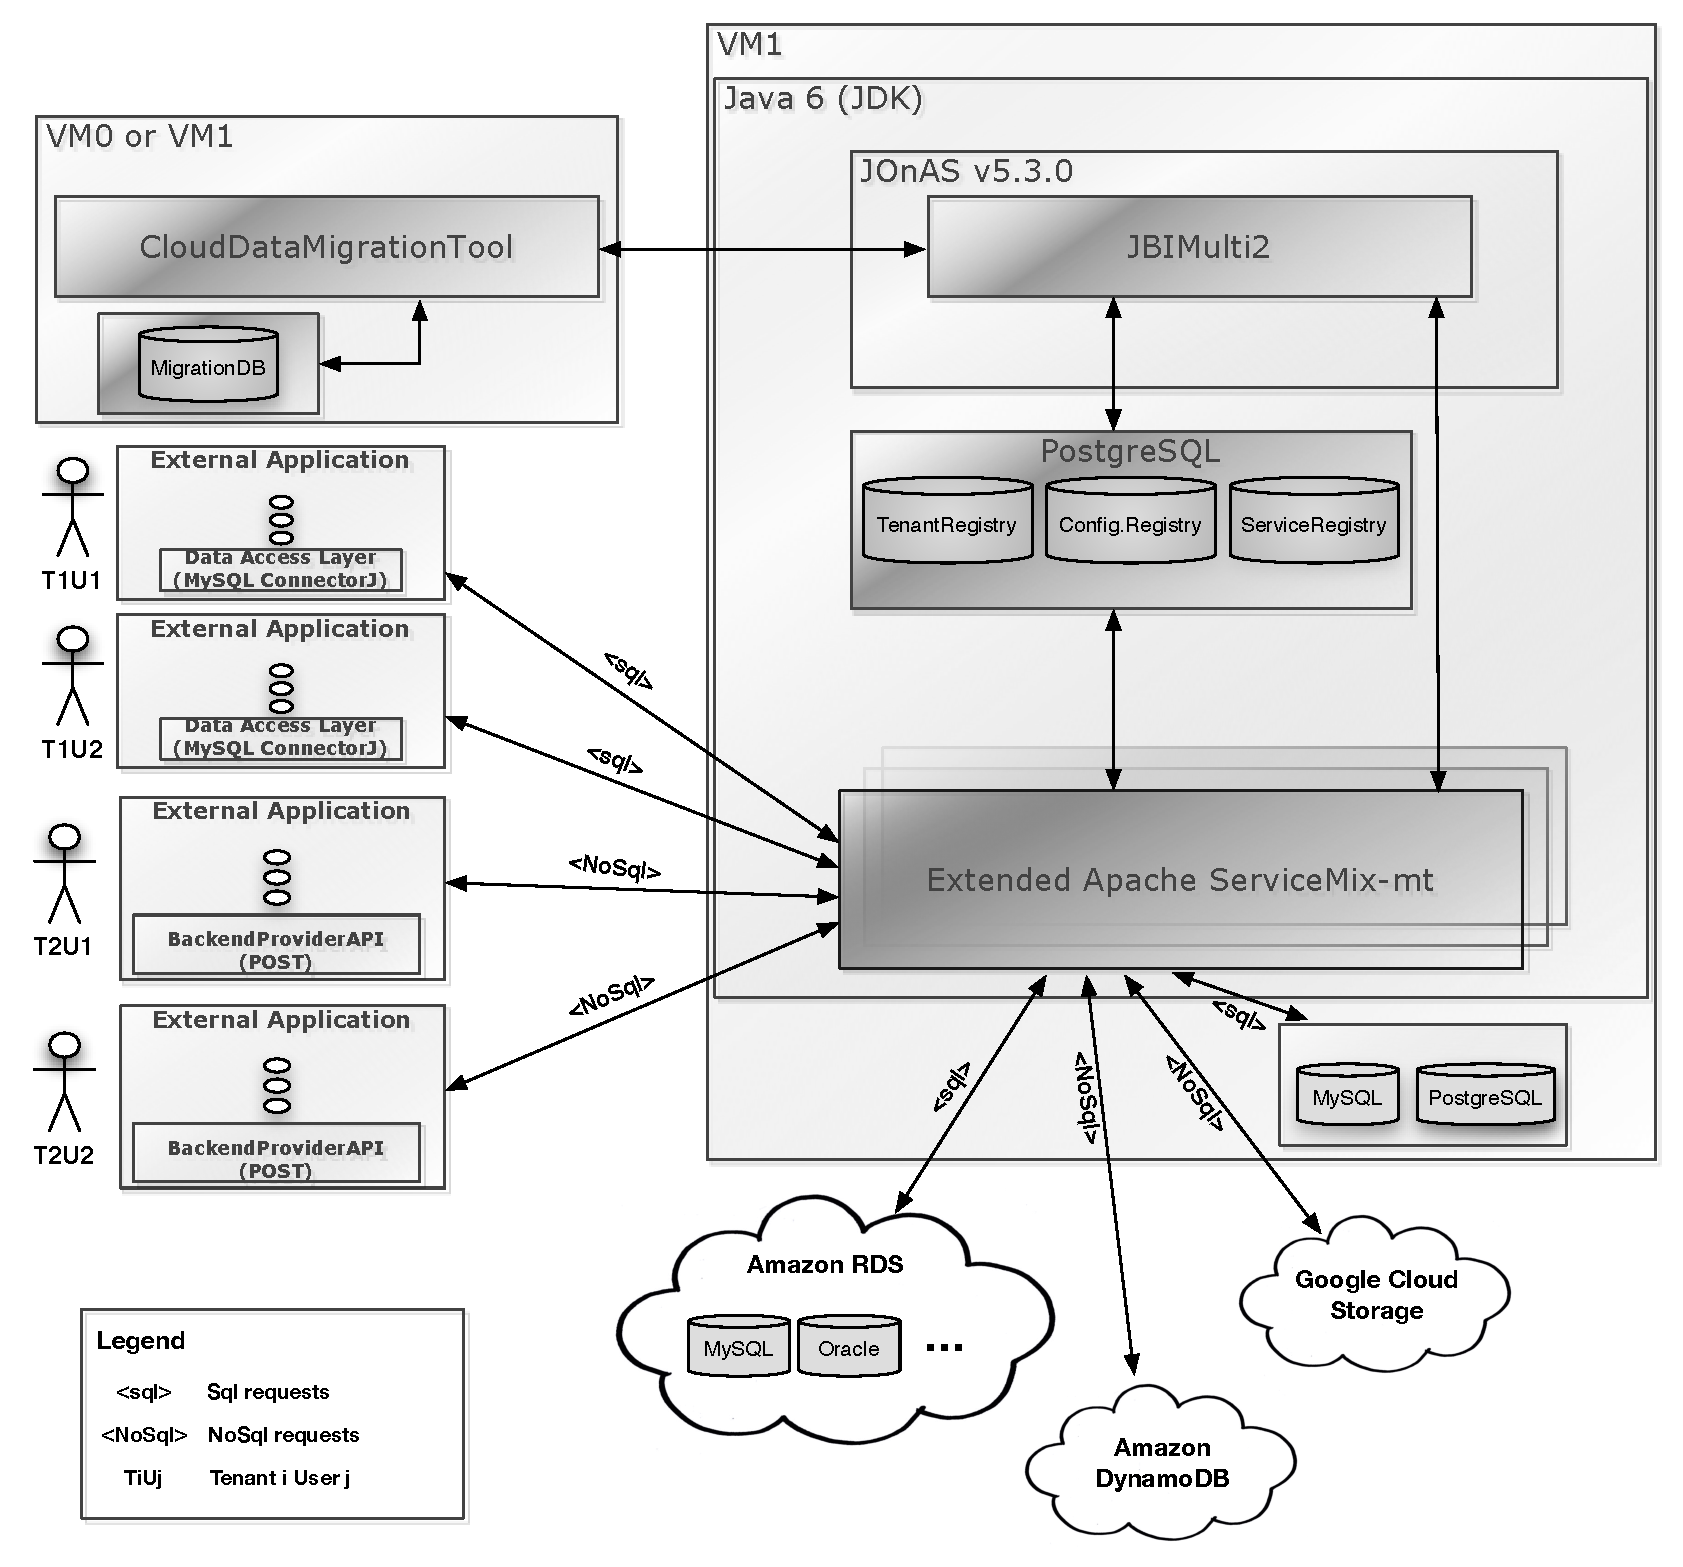
\includegraphics[clip, scale=0.5]{./gfx/systemoverview.pdf}
	\caption[Transparent Cloud Data Access System Overview]{Transparent Cloud data access system overview, including the \term{Cloud Data Migration Application} \cite{bachmann2012}. Note: represents the system in the post-migration phase}
	\label{fig:systemoverview}
\end{figure}

The transparent Cloud data access access support is achieved by the interaction of three main components: JBIMulti2, registries containing tenant-aware information, and an extended version of ServiceMix-mt (see Figure \ref{fig:systemoverview}). JBIMulti2 deploys in ServiceMix-mt the \ac{SA}s containing the endpoint and routing configurations selected by the tenant, which support two different communication protocols: MySQL and \ac{HTTP}. From this point the DAL of the tenant's application can retrieve and modify data in his data container in the Cloud through the \ac{ESB} connecting to a single logical endpoint which connects to multiple physical backend data stores. In our approach we provide also the possibility, either to configure a connection to the traditional database, e.g. when a hybrid model is pursued, or to utilize a \ac{DBMS} provided in our system, which is described in the following subsection.

%The JBIMulti2 utilizes three main components in the system: registries created in a PostgreSQL database, resources in ActiveMQ and ServiceMix. When deploying a tenant's \ac{SA} the application initiates an unidirectional communication to a management queue from which a management \ac{OSGi} bundle consumes the management messages from JBIMulti2 and performs managements operations in ServiceMix, such as deploy and undeploy. The deployed multi-tenant \ac{SA}s configure the tenants' endpoints for \ac{BC}s or \ac{SE}s. When deployed a multi-tenant \ac{SA} which packages a \ac{JMS} endpoint configuration, resources are transparently created in the out-of-the-box ActiveMQ instance which is shipped with ServiceMix. However, it is out of the scope of this student thesis an interface for connecting the different tenants with the created \ac{JMS} resources.


\FloatBarrier
\newpage
\section{Funktionsweise des Ansatzes}
\label{sec:FunktionsweiseAnsatz}

In Figure \ref{fig:componentoverview} we specify the main components which build the subsystem mentioned in Section \ref{sec:systemoverview}. We highlight the components which require an extension, and the new components which are implemented and included in the system. 

\begin{figure}[htb]
	\centering
		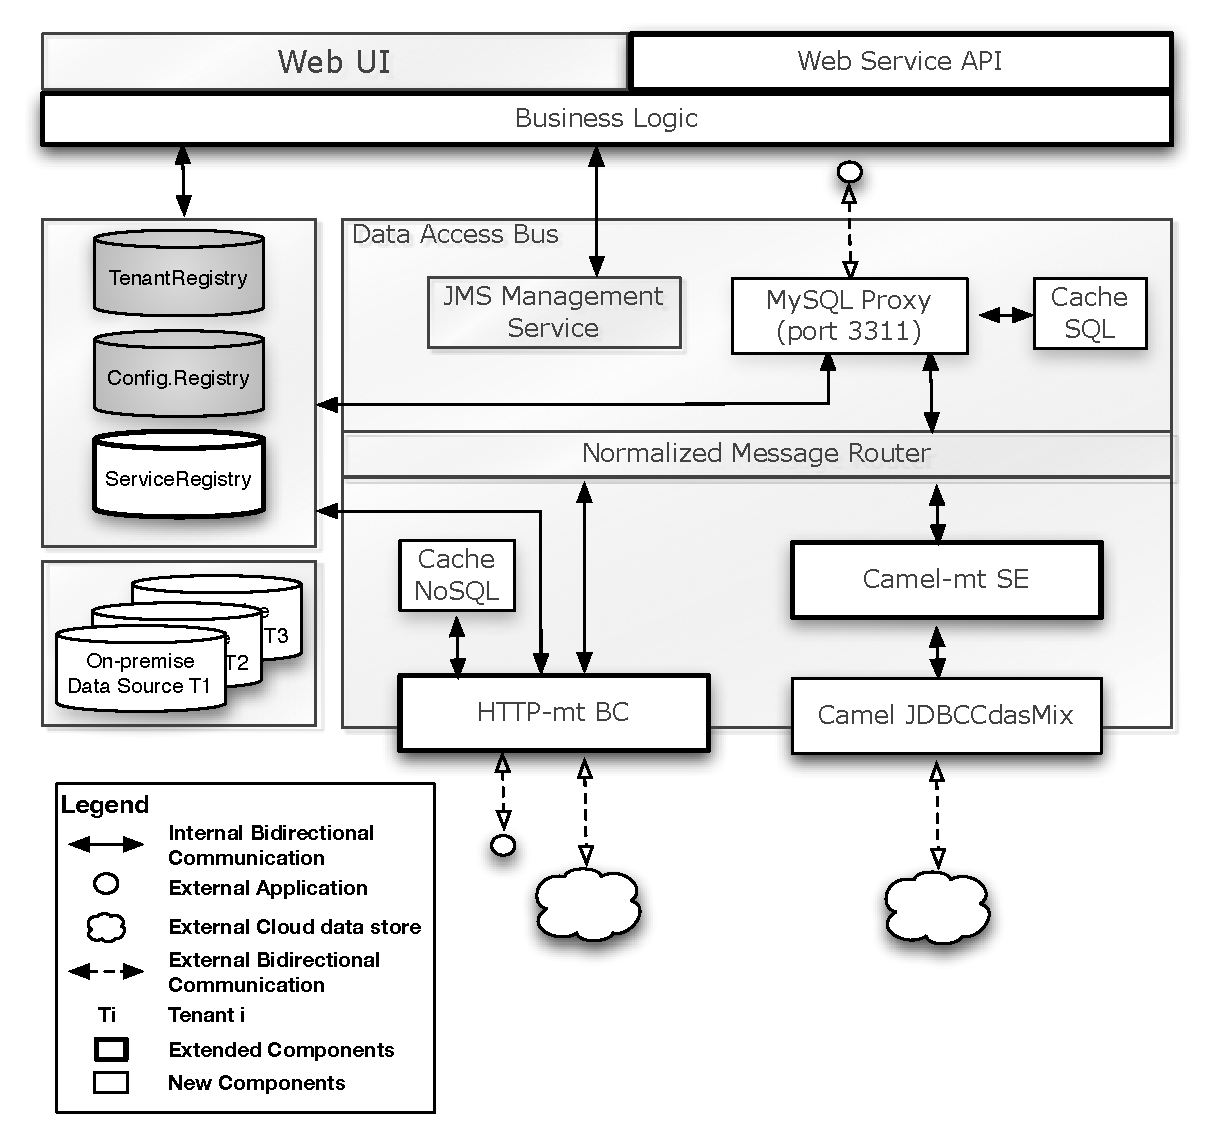
\includegraphics[clip, scale=0.6]{./gfx/componentoverview.pdf}
	\caption[Transparent Cloud Data Access Components Overview]{Transparent Cloud data access components overview.}
	\label{fig:componentoverview}
\end{figure}

As described in Section \ref{sec:systemoverview}, we extend the JBIMulti2 Web service \ac{API} and its associated business logic. The operations we include perform access and modifications to one particular registry: the Service Registry. This registry persists information about services, its policies, and \ac{SA}s deployed by one tenant. The last kind of information is the one we mainly focus on, due to the information which is contained in it: the tenant-aware endpoint configuration in ServiceMix-mt. Therefore, we extend this registry to persist the configuration about the data stores. We make a differentiation between data stores and name it source and target data sources, to be able to relate the one that the tenant physically accesses and the one which the tenant logically accesses, which is the one that the system physically accesses. To support transparent access to two different database types, we divide our architecture and implementation into the the communication protocols they support: MySQL for MySQL databases, and HTTP for \ac{NoSQL} databases (see Figure \ref{fig:componentoverview}). 

For the first one, the single access physical endpoint is provided through a \ac{TCP} port, which then forwards the message to the appropriate tenant's endpoint in the multi-tenant Servicemix Camel component, and this to the component which physically connects to the backend \ac{SQL} \ac{DBMS}. For the second one, we extend the Servicemix-http-mt in order to physically connect to the backend \ac{NoSQL} data stores. 

The possibility of migrating a database to the VM instance where the \ac{ESB} runs is also supported. However, we do not provide a multi-tenant \ac{DBMS} where a database or table is shared between multiple tenants, since it is not a requirement in this diploma thesis. The ensured isolation in this case is the one provided by a \ac{DBMS} between different databases. Furthermore, backup, restoration, administration, and horizontal scalability services are not supported. We provide in the VM instance where CDASMix runs a MySQL database system. The number and types of databases systems supported in the VM instance relies on the administrator, and the PostgreSQL database system where the system registries are stored must be independent from the PostgreSQL instance which hosts the migrated tenant's databases.

As represented in Figure \ref{fig:componentoverview}, we enhance ServiceMix-mt with cashing support, in particular for the two different types of databases we support. The cashing mechanism supports storage of access control data, as well as retrieved data from the backend data store, e.g. a bucket, or a set of rows. The reasons for using a divided cashing system instead of a single one is explained in Chapter \ref{chap:design}. 

\FloatBarrier

\chapter{Implementierung einer Teilmenge ausgewählten Ansätzen}
\label{chap:Implementierung}

%In this chapter we present the architectural and technological solution taken into account to integrate two approaches for enabling multi-tenancy in a \ac{ESB} solution \cite{Essl2011}, \cite{Muhler2012}. Furthermore, it fulfills the requirements described in the Chapter \ref{chap:spec} and provides a detailed design for easing the implementation cycle described in Chapter \ref{chap:implementation}. We start defining the architecture of the prototype we should implement in this thesis and we continue by giving more details on specific components that need to be extended or modified. As discussed in the previous chapters, some communication approaches taken into account in the master's thesis \cite{Essl2011} need to be improved. When describing them, we specify the main differences and the main advantages of the design approach we take. 

In this chapter we present the architectural solution taken into account to build the system which fulfills the requirements specified in Chapter \ref{chap:spec}. Due to the required communication support for \ac{SQL} and \ac{NoSQL} databases, we separate the architectural approaches and provide them separately. JBIMulti2 and ServiceMix-mt are the subsystems we must reengineer in order to aggregate transparent and dynamic routing functionalities. Therefore, we also provide in this chapter the needed extensions in the components conforming the system, e.g. service registry in JBIMulti2, and \ac{NMF} in ServiceMix-mt.



\FloatBarrier
\input{implementation/Evaluierung}
\chapter{zusammenfassung und Ausblick}
\label{chap:zusammenfassung}

%In order to ensure that  we fulfill the requirements listed in Chapter \ref{chap:spec}, in this chapter we provide a testing of the main components we implemented and we describe how we initialize the different testing scenarios. In Section \ref{sec:multitenanttest} we provide three different testing scenarios, one per extended \ac{BC}, and we monitor both incoming and outgoing messages to and from the \ac{ESB}.

In this chapter we provide the validation, and evaluation of the system. We must ensure that the requirements specified in Chapter \ref{chap:spec} are fulfilled in the design and implementation phases. In Section \ref{sec:deploymentandinit} we describe the steps which should be followed to initialize the system, and the testing scenarios. After the initialization we execute the test cases in Section \ref{sec:validation}, and monitor the incoming requests to ServiceMix-mt, and the outgoing requests to the backend Cloud data store. Due to the extensions implemented on the \ac{ESB}, we evaluate in Section \ref{sec:evaluation} its behavior, and the impact that our modifications have on the original ServiceMix-mt.



\begin{appendix}


\chapter{Components}

%This chapter lists \ac{XSD}s that WS-Policy Assertion language and Rules XML file must conform. Furthermore, there are given several policy documents of Cloud data stores that are used for validation.

\section{CDASMix MySQL Proxy}
\label{appendix:cdasmixmysqlproxy}

The MySQL proxy \ac{OSGi} bundle is implemented on the Continuent Tungsten Connector \cite{tungstenwiki}, which is a Java MySQL proxy which directly connects with the backend MySQL database system. We extend and adapt this proxy in order to integrate it with ServiceMix, aggregate transparency, multi-tenant awareness, cashing, and dynamic connection with the backend Cloud data sources.

\begin{figure}[htb]
	\centering
		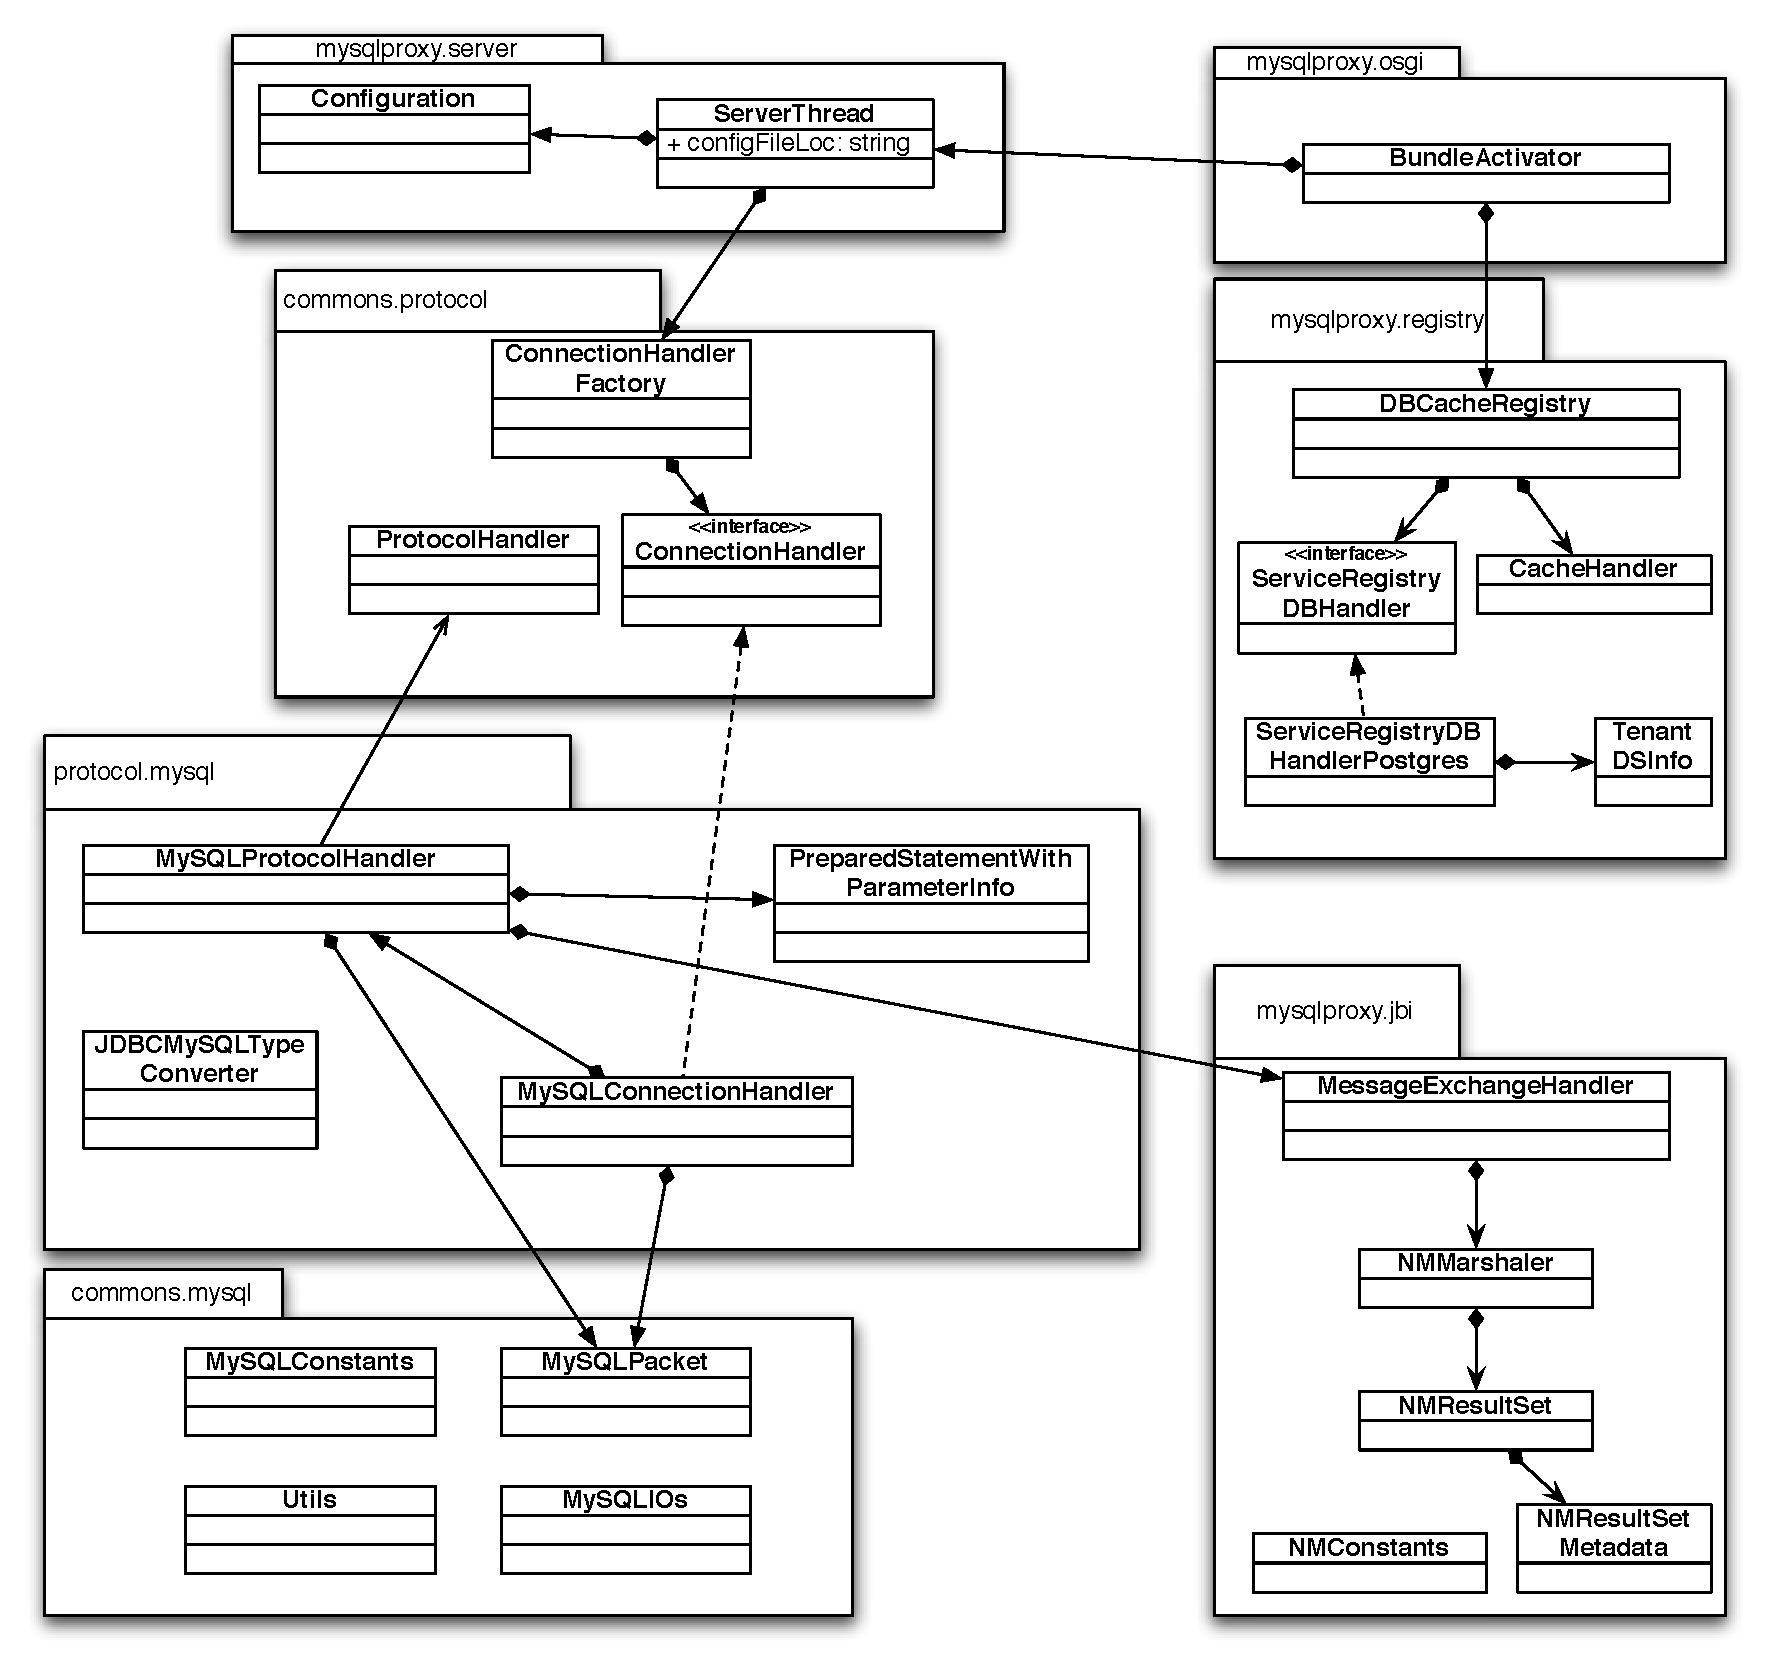
\includegraphics[clip, scale=0.4]{./gfx/mysql-osgi/mysql-proxy-v3.pdf}
	\caption[ServiceMix-mt MySQL OSGi Bundle]{OSGi bundle providing MySQL support in ServiceMix-mt}
	\label{fig:mysqlclassdiagram}
\end{figure}

\FloatBarrier

\vspace*{0.5cm}

%\lstinputlisting[label={lst:policy_language_syntax},caption={[Syntax of WS-Policy Assertion Language Schema]Syntax of WS-Policy Assertion Language Schema.},style=xml]{./gfx/master_thesis/cdhs-ws.xml}

%\vspace*{1cm}

%\vspace*{0.5cm}

%\lstinputlisting[label={lst:policy_language_schema},caption={[CDHS WS-Policy Assertion Language Schema]CDHS WS-Policy Assertion Language Schema.},style=xml]{./gfx/master_thesis/cdhs_properties.xsd}

%\vspace*{1cm}

\section{CDASMix Camel JDBC}
\label{subsec:cdasmixcameljdbc}

The \term{cdasmixjdbc} component is a custom component which is built and deployed as an \ac{OSGi} bundle in ServiceMix-mt. It provides support for connections with backend \ac{SQL} Cloud data stores, and message marshaling and demarshaling.

\begin{sidewaysfigure}[htb]
	\centering
		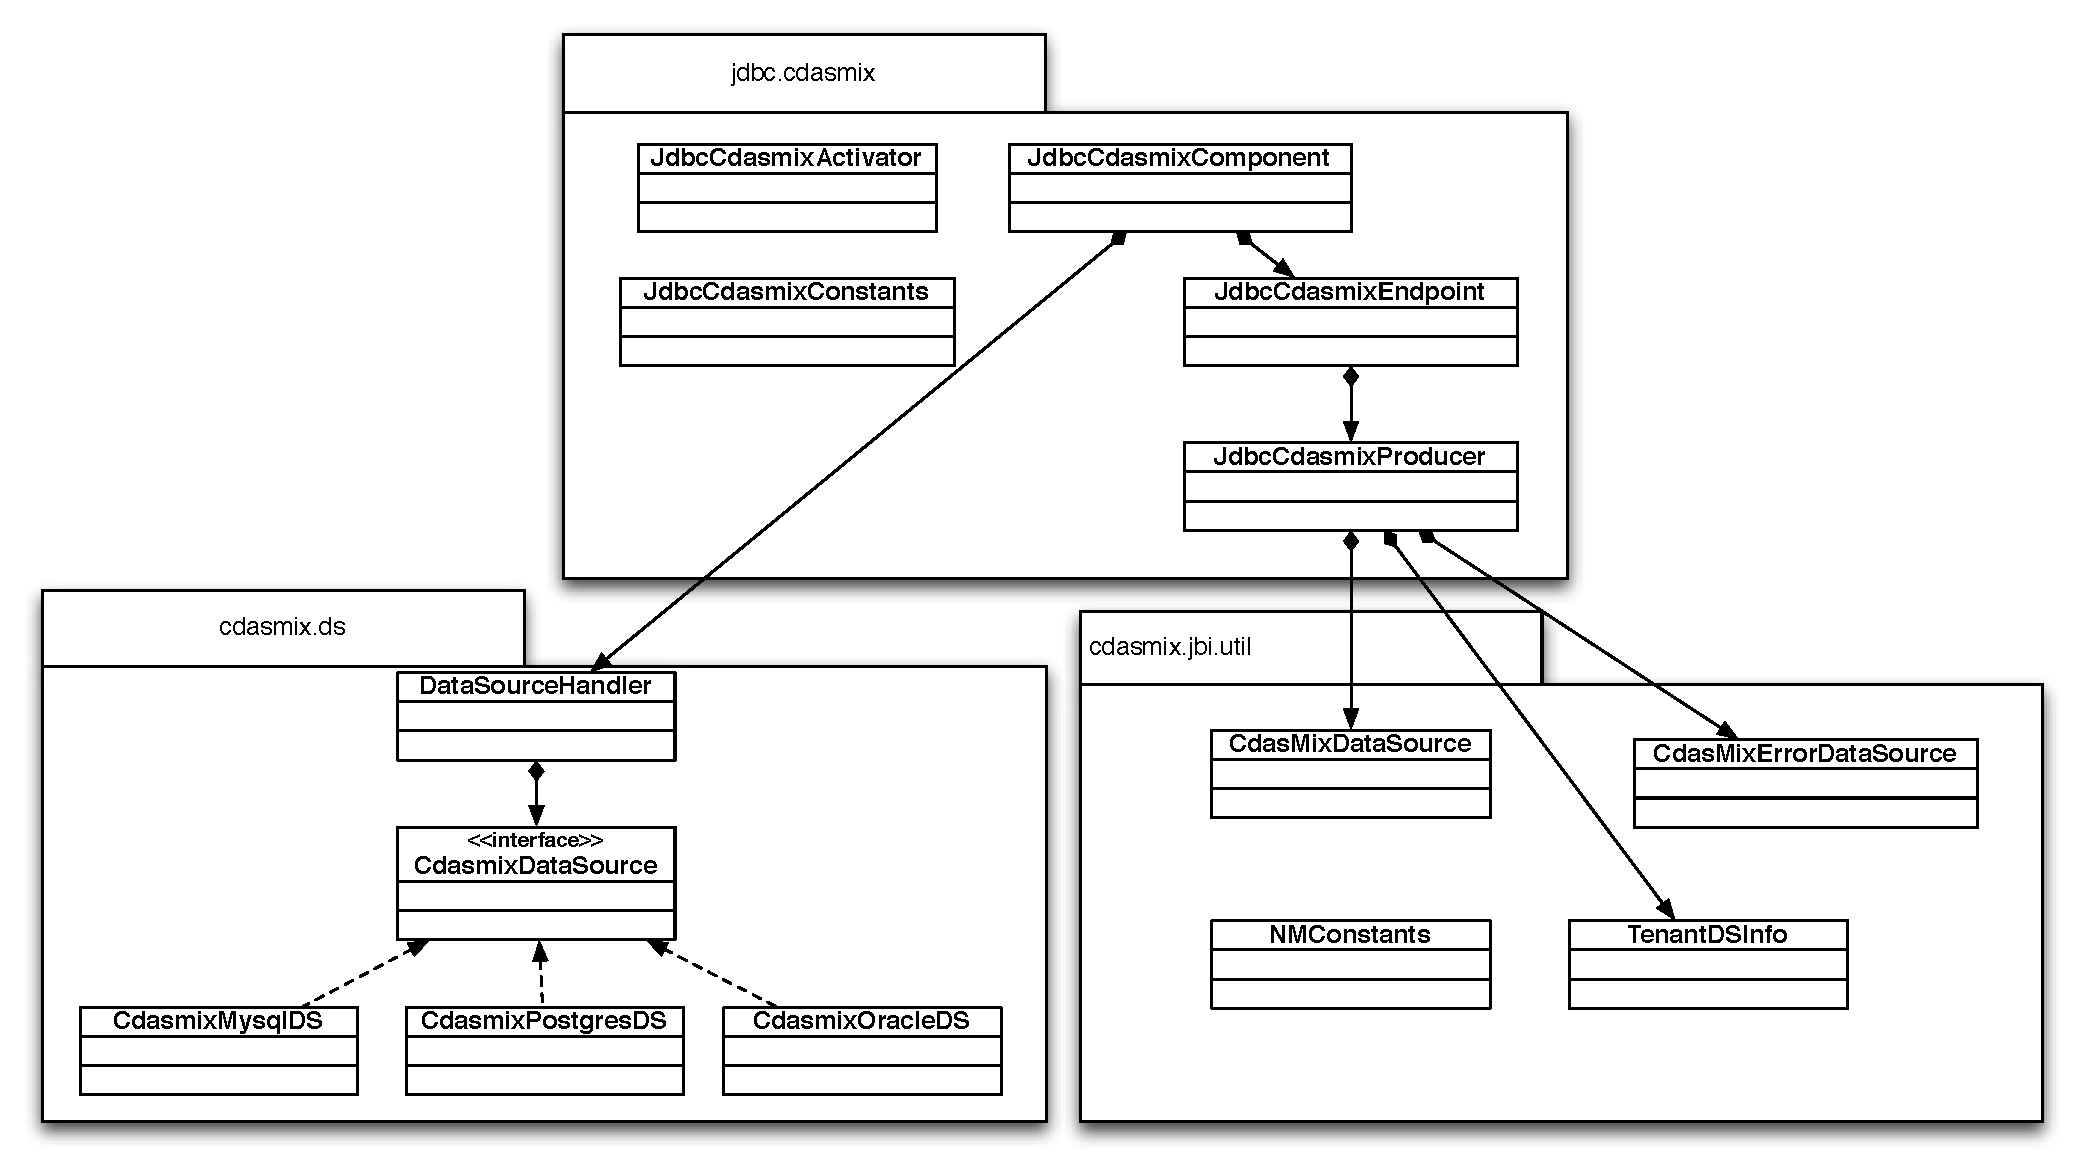
\includegraphics[clip, scale=0.6]{./gfx/cdasmix-camel-jdbc/cdasmix-camel-jdbc.pdf}
	\caption[ServiceMix-mt Camel CDASMix-JDBC Component]{OSGi bundle and Camel component providing JDBC support in ServiceMix-mt}
	\label{fig:cdasmixjdbcclassdiagram}
\end{sidewaysfigure}

\vspace*{0.5cm}

\FloatBarrier

%\lstinputlisting[label={lst:rules_schema},caption={[Post-Processing Rules XML Schema]Post-Processing Rules XML Schema.},style=xml]{./gfx/master_thesis/rules.xsd}

%\vspace*{1cm}

%\section{Multi-tenant ServiceMix HTTP Binding Component}
%\label{appendix:httpmtbc}

%to be filled
%\vspace*{0.5cm}

%\lstinputlisting[label={lst:googleCloudSQL-policy},caption={[Google Cloud SQL Service Provider Policy]Google Cloud SQL Service Provider Policy.},style=xml]{./gfx/master_thesis/provider_policies/GoogleCloudSQL.wspolicy}

%\vspace*{1cm}

%\vspace*{0.5cm}

%\lstinputlisting[label={lst:sqlDatabase-policy},caption={[SQL Database Service Provider Policy]SQL Database Service Provider Policy.},style=xml]{./gfx/master_thesis/provider_policies/SQLDatabase.wspolicy}

%\vspace*{1cm}
\FloatBarrier


\clearpage
\chapter{Messages}

%This chapter lists \ac{XSD}s that WS-Policy Assertion language and Rules XML file must conform. Furthermore, there are given several policy documents of Cloud data stores that are used for validation.
In this chapter we provide an overview of the requests which are sent to, and received from the extended ServiceMix-mt. For MySQL requests we provide the \ac{TCP} packets which are transferred between the application, ServiceMix-mt, and the backend MySQL database system. For NoSQL requests we present messages samples which are in \ac{JSON} format, but its content varies among the different backend Cloud data store providers. 

\section{Normalized Message Format Content Description}
\label{appendix:nmfcontent}

In this section we provide an overview of the data structures which are sent in the \ac{NMF}. The sections of the \ac{NMF} where the data and meta-data are sent are the \term{properties}, and the \term{attachment}.  In the Listing \ref{lst:nmfcontent} we detail the contents sent in each of the sections, and the data structures in which the data and meta-data are stored.

%\vspace*{0.5cm}

%\lstinputlisting[label={lst:policy_language_syntax},caption={[Syntax of WS-Policy Assertion Language Schema]Syntax of WS-Policy Assertion Language Schema.},style=xml]{./gfx/master_thesis/cdhs-ws.xml}

%\vspace*{1cm}
\vspace*{0.5cm}
%%%%%%%%%%%%%%%%%%%%%%%%%%%%%
\lstinputlisting[label={lst:nmfcontent},caption={[Data and Meta-data Detail in the Normalized Message Format]Detail of the content and data structures used to send the requests' data and meta-data.},style=ebnf]{./gfx/NMF_v3_0.txt}
%%%%%%%%%%%%%%%%%%%%%%%%%%%%%
\vspace*{1cm}

\section{MySQL TCP Stream}
\label{appendix:messagemysql}

In this section we provide two \ac{TCP} streams which are captured with the \term{ngrep} program for UNIX \cite{ngrep}. The first stream captures the \ac{TCP} packets on port 3311, where the MySQL component in ServiceMix-mt listens for incoming connections (see Listing \ref{lst:tcpstream3311}). The second stream captures the \ac{TCP} packets on port 3306, where the a locally deployed MySQL server listens for incoming connections (see Listing \ref{lst:tcpstream3306}).

%%%%%%%%%%%%%%%%%%%%%%%%%%%%%
\lstinputlisting[float=htb,label={lst:tcpstream3311},caption={[TCP Stream for a MySQL Communication Captured on Port 3311]TCP Stream for a MySQL communication captured on port 3311 with the program \term{ngrep} \cite{ngrep}.},style=ebnf]{./gfx/tcpstreamoutput3311.txt}
%%%%%%%%%%%%%%%%%%%%%%%%%%%%%

%%%%%%%%%%%%%%%%%%%%%%%%%%%%%
\lstinputlisting[float=htb,label={lst:tcpstream3306},caption={[TCP Stream for a MySQL Communication Captured on Port 3306]TCP Stream for a MySQL communication captured on port 3306 with the program \term{ngrep} \cite{ngrep}.},style=ebnf]{./gfx/tcpstream3306.txt}
%%%%%%%%%%%%%%%%%%%%%%%%%%%%%

\vspace*{0.5cm}

%\lstinputlisting[label={lst:policy_language_syntax},caption={[Syntax of WS-Policy Assertion Language Schema]Syntax of WS-Policy Assertion Language Schema.},style=xml]{./gfx/master_thesis/cdhs-ws.xml}

\vspace*{1cm}

\vspace*{0.5cm}

%\lstinputlisting[label={lst:policy_language_schema},caption={[CDHS WS-Policy Assertion Language Schema]CDHS WS-Policy Assertion Language Schema.},style=xml]{./gfx/master_thesis/cdhs_properties.xsd}

\vspace*{1cm}

\FloatBarrier


%\section{JSON in POST Request}
%\label{subsec:jsonpost}

%to be filled

\vspace*{0.5cm}

%\lstinputlisting[label={lst:rules_schema},caption={[Post-Processing Rules XML Schema]Post-Processing Rules XML Schema.},style=xml]{./gfx/master_thesis/rules.xsd}

\vspace*{1cm}

\FloatBarrier

\clearpage

\end{appendix}
\bibliographystyle{alphancex}
%\bibliography{literatur/literatur}

\bibliography{literatur/Literatur_Mpessa}

All links were last followed on March 21, 2013.

\clearpage
\pagestyle{empty}
\vspace{9cm}
\begin{center}
\begin{minipage}{11cm}
\vspace{6cm}

\textbf{\Large Acknowledgement}\\\\
I am heartily thankful to my supervisor Steve Strauch from the University of Stuttgart for his encouragement, guidance and support in all the phases of this diploma thesis. I am also grateful to Dr. Vasilios Andrikopoulos for his advices and useful tips.
Special thanks to my family, friends and girlfriend for their moral support.

\vspace{1cm}
Santiago G\'omez S\'aez

\end{minipage}
\end{center}

\clearpage
\pagestyle{empty}
\vspace{9cm}
\begin{center}
\begin{minipage}{11cm}
\vspace{6cm}

\textbf{\Large Declaration}\\\\
\vspace{0.4cm}

All the work contained within this thesis,
except where otherwise acknowledged, was
solely the effort of the author. At no
stage was any collaboration entered into
with any other party.
\vspace{1cm}

Stuttgart, 22nd March 2013 \hspace{1cm}--------------------------------\\
\phantom{Stuttgart, March 22 2013} \hspace{1.3cm} (Santiago G\'omez S\'aez)
\end{minipage}
\end{center}

\end{document}
